% Options for packages loaded elsewhere
\PassOptionsToPackage{unicode}{hyperref}
\PassOptionsToPackage{hyphens}{url}
\PassOptionsToPackage{dvipsnames,svgnames*,x11names*}{xcolor}
%
\documentclass[
]{article}
\usepackage{amsmath,amssymb}
\usepackage{lmodern}
\usepackage{ifxetex,ifluatex}
\ifnum 0\ifxetex 1\fi\ifluatex 1\fi=0 % if pdftex
  \usepackage[T1]{fontenc}
  \usepackage[utf8]{inputenc}
  \usepackage{textcomp} % provide euro and other symbols
\else % if luatex or xetex
  \usepackage{unicode-math}
  \defaultfontfeatures{Scale=MatchLowercase}
  \defaultfontfeatures[\rmfamily]{Ligatures=TeX,Scale=1}
\fi
% Use upquote if available, for straight quotes in verbatim environments
\IfFileExists{upquote.sty}{\usepackage{upquote}}{}
\IfFileExists{microtype.sty}{% use microtype if available
  \usepackage[]{microtype}
  \UseMicrotypeSet[protrusion]{basicmath} % disable protrusion for tt fonts
}{}
\makeatletter
\@ifundefined{KOMAClassName}{% if non-KOMA class
  \IfFileExists{parskip.sty}{%
    \usepackage{parskip}
  }{% else
    \setlength{\parindent}{0pt}
    \setlength{\parskip}{6pt plus 2pt minus 1pt}}
}{% if KOMA class
  \KOMAoptions{parskip=half}}
\makeatother
\usepackage{xcolor}
\IfFileExists{xurl.sty}{\usepackage{xurl}}{} % add URL line breaks if available
\IfFileExists{bookmark.sty}{\usepackage{bookmark}}{\usepackage{hyperref}}
\hypersetup{
  pdftitle={Political news coverage of online news},
  pdfauthor={Franziska Löw},
  colorlinks=true,
  linkcolor=blue,
  filecolor=Maroon,
  citecolor=Blue,
  urlcolor=Blue,
  pdfcreator={LaTeX via pandoc}}
\urlstyle{same} % disable monospaced font for URLs
\usepackage[margin=1in]{geometry}
\usepackage{longtable,booktabs,array}
\usepackage{calc} % for calculating minipage widths
% Correct order of tables after \paragraph or \subparagraph
\usepackage{etoolbox}
\makeatletter
\patchcmd\longtable{\par}{\if@noskipsec\mbox{}\fi\par}{}{}
\makeatother
% Allow footnotes in longtable head/foot
\IfFileExists{footnotehyper.sty}{\usepackage{footnotehyper}}{\usepackage{footnote}}
\makesavenoteenv{longtable}
\usepackage{graphicx}
\makeatletter
\def\maxwidth{\ifdim\Gin@nat@width>\linewidth\linewidth\else\Gin@nat@width\fi}
\def\maxheight{\ifdim\Gin@nat@height>\textheight\textheight\else\Gin@nat@height\fi}
\makeatother
% Scale images if necessary, so that they will not overflow the page
% margins by default, and it is still possible to overwrite the defaults
% using explicit options in \includegraphics[width, height, ...]{}
\setkeys{Gin}{width=\maxwidth,height=\maxheight,keepaspectratio}
% Set default figure placement to htbp
\makeatletter
\def\fps@figure{htbp}
\makeatother
\setlength{\emergencystretch}{3em} % prevent overfull lines
\providecommand{\tightlist}{%
  \setlength{\itemsep}{0pt}\setlength{\parskip}{0pt}}
\setcounter{secnumdepth}{-\maxdimen} % remove section numbering
\usepackage{float}
\usepackage{pdflscape}
\newcommand{\blandscape}{\begin{landscape}}
\newcommand{\elandscape}{\end{landscape}}
\usepackage{subfig}
\usepackage{booktabs}
\usepackage{longtable}
\usepackage{array}
\usepackage{multirow}
\usepackage{wrapfig}
\usepackage{float}
\usepackage{colortbl}
\usepackage{pdflscape}
\usepackage{tabu}
\usepackage{threeparttable}
\usepackage{threeparttablex}
\usepackage[normalem]{ulem}
\usepackage{makecell}
\usepackage{xcolor}
\ifluatex
  \usepackage{selnolig}  % disable illegal ligatures
\fi
\newlength{\cslhangindent}
\setlength{\cslhangindent}{1.5em}
\newlength{\csllabelwidth}
\setlength{\csllabelwidth}{3em}
\newenvironment{CSLReferences}[2] % #1 hanging-ident, #2 entry spacing
 {% don't indent paragraphs
  \setlength{\parindent}{0pt}
  % turn on hanging indent if param 1 is 1
  \ifodd #1 \everypar{\setlength{\hangindent}{\cslhangindent}}\ignorespaces\fi
  % set entry spacing
  \ifnum #2 > 0
  \setlength{\parskip}{#2\baselineskip}
  \fi
 }%
 {}
\usepackage{calc}
\newcommand{\CSLBlock}[1]{#1\hfill\break}
\newcommand{\CSLLeftMargin}[1]{\parbox[t]{\csllabelwidth}{#1}}
\newcommand{\CSLRightInline}[1]{\parbox[t]{\linewidth - \csllabelwidth}{#1}\break}
\newcommand{\CSLIndent}[1]{\hspace{\cslhangindent}#1}

\title{Political news coverage of online news}
\usepackage{etoolbox}
\makeatletter
\providecommand{\subtitle}[1]{% add subtitle to \maketitle
  \apptocmd{\@title}{\par {\large #1 \par}}{}{}
}
\makeatother
\subtitle{\ldots{}}
\author{Franziska Löw\footnote{Institut für Industrieökonomik, Helmut
  Schmidt Universität. Email: .}}
\date{November 2020}

\begin{document}
\maketitle

\hypertarget{i-introduction}{%
\section{I Introduction}\label{i-introduction}}

In democracies, the media fulfill fundamental functions: They should
inform the people, contribute to the formation of opinion through
criticism and discussion and thus enable participation. In recent
decades, however, concern has grown about the role of the media in
politics in general and in election campaigns in particular. They are
criticized for influencing election results through their reporting and
for helping populist parties in particular to flourish. After the 2017
federal elections in Germany, for example, the media were accused of
contributing to the success of the right-wing populist AfD by
increasingly including the party's content and using the same language
in their articles as the AfD. Representatives of these media houses
strongly opposed this accusation. The purpose of this study is to
examine whether there is evidence that supports the accusation of biased
media reporting, especially during election campaigns.

For advertising-financed media the battle for the attention of the
recipients is at the center of economic decisions. Online media in
particular, which offer their content to a large extent free of charge
and generate their revenue through advertising space, compete for the
scarce resource of attention. Consumers pay a non-monetary price
providing their attention, which the media platform bundles and sells on
to advertising customers. This business model corresponds to that of a
platform market, in which media companies act as platforms that connect
the market of advertising with the reader market to exploit the indirect
network effects between them
(\protect\hyperlink{ref-dewenter_einfuhrung_2014}{Dewenter and Rösch
2014}). A profit-maximizing publisher therefore directs its economic
decisions according to what will attract the most attention.

This conclusion, derived from the economic theory of platform markets,
corresponds to the notion of media logic, a central concept in the field
of media and communication studies
(\protect\hyperlink{ref-takens_media_2013}{Takens et al. 2013}). The
debate about media logic is embedded in the broader discussion about the
interaction between the press, politics and the public. The underlying
thesis is that the content of political news is the product of news
values and narrative techniques that media use to attract audiences
(\protect\hyperlink{ref-stromback_four_2008}{Strömbäck 2008}). According
to \protect\hyperlink{ref-takens_media_2013}{Takens et al.}
(\protect\hyperlink{ref-takens_media_2013}{2013}), three content
attributes highly correspond with news values and influence how
journalists interpret political events: 1) personalized content, i.e.,
the focus on individual politicians; 2) the framing of politics as a
contest and 3) negative coverage. Similarly
\protect\hyperlink{ref-blassnig_hitting_2019}{Blassnig et al.}
(\protect\hyperlink{ref-blassnig_hitting_2019}{2019}) states that media
primarily focus on news factors, i.e.~the factors that turn an event
into news worth reporting like conflict, drama, negativity, surprise or
proximity. Likewise populist messages often co-occur with negative,
emotionalized, or dramatized communication style, thus utilizing similar
mechanisms as the media logic, respectively the attention economy. In
fact, \protect\hyperlink{ref-blassnig_hitting_2019}{Blassnig et al.}
(\protect\hyperlink{ref-blassnig_hitting_2019}{2019}) shows that
populist key messages by political and media actors in news articles
provoke more reader comments under these articles. Media competing for
the attention of readers therefore have an incentive to pick up on the
key messages of these parties. These, in turn, benefit from being able
to place their agendas in the public debate
(\protect\hyperlink{ref-druckman_impact_2005}{Druckman and Parkin}
(\protect\hyperlink{ref-druckman_impact_2005}{2005}),
\protect\hyperlink{ref-eberl_lying_2018}{Eberl}
(\protect\hyperlink{ref-eberl_lying_2018}{2018})). It is assumed, that
smaller, non-established parties in particular benefit from placing
their topics in the media in order to get them into the voters' heads.
Here, the tendency of the reporting is irrelevant but rather the
quantity is decisive.

However, the causal relationship between reporting and voter preferences
is not the subject of this study. Rather, it is intended to measure how
online news coverage coincides with the messaging of different political
parties. Especially during election campaigns political parties want the
media agenda to be congruent with their own agenda to define the
issue-based criteria on which they will be evaluated by voters
(\protect\hyperlink{ref-eberl_one_2017}{Eberl, Boomgaarden, and Wagner
2017}). Parties instrumentalize their public relations in order to
highlight issues that they are perceived to be competent on, that they
``own'' and that are important to their voters
(\protect\hyperlink{ref-kepplinger_einfluss_2004}{Kepplinger and Maurer
2004}). This paper therefore analyzes the period before and after the
2017 federal elections in Germany to answer the question whether
political news report about similar topics and if this similarity
changes after the election campaign is over.

In order to answer these and other media-related questions in the
political context, quantifying the content of media is a prerequisite.
One of the key challenges is to determine the features that are used to
describe media content - be it audio, video or text content. Studies
that rely on quantifying media content for their analyses use, for
example, visibility (how often political actors appear in the media) or
tonality (how they are evaluated). Other studies examine the topics
discussed or the language used in the media, in order to identify
whether political actors are able to place their own policy positions in
the media. Leading studies from economic literature, for example,
examine how often a newspaper quotes the same think tanks
(\protect\hyperlink{ref-groseclose_measure_2005}{Groseclose and Milyo}
(\protect\hyperlink{ref-groseclose_measure_2005}{2005}),
\protect\hyperlink{ref-lott_is_2014}{Lott and Hassett}
(\protect\hyperlink{ref-lott_is_2014}{2014})) or uses the same language
(\protect\hyperlink{ref-gentzkow_media_2004}{M. A. Gentzkow and Shapiro
2004}) as members of Congress. Following this approach, the present
paper compares topics discussed in media outlets with topics addressed
in the press releases of the parties in the German ``Bundestag,'' to
measure the content similarity between online news and parties press
releases.\footnote{For the sake of simplicity, both news articles and
  press releases will be referred to as documents in the following.} To
discover the latent topics in the corpus of text data, the structural
topic model (STM) developed by
\protect\hyperlink{ref-roberts_model_2016}{M. E. Roberts, Stewart, and
Airoldi} (\protect\hyperlink{ref-roberts_model_2016}{2016}) is applied.
This probabilistic text model results in a probability distribution for
each document across all topics, which is then aggregated to calculate
the degree of difference between the news articles of different media
providers and the press releases of the parties using a linear
regression model.

The figure below gives a high level overview of the research method: 1.
in section III: explain which data is used and how the text is processed
in order to use it as input for the structural topic model. 2. in
section IV: explains how the cosine similarity between documents is
calculated using the output of the structural topic model 3. in section
V: model estimation

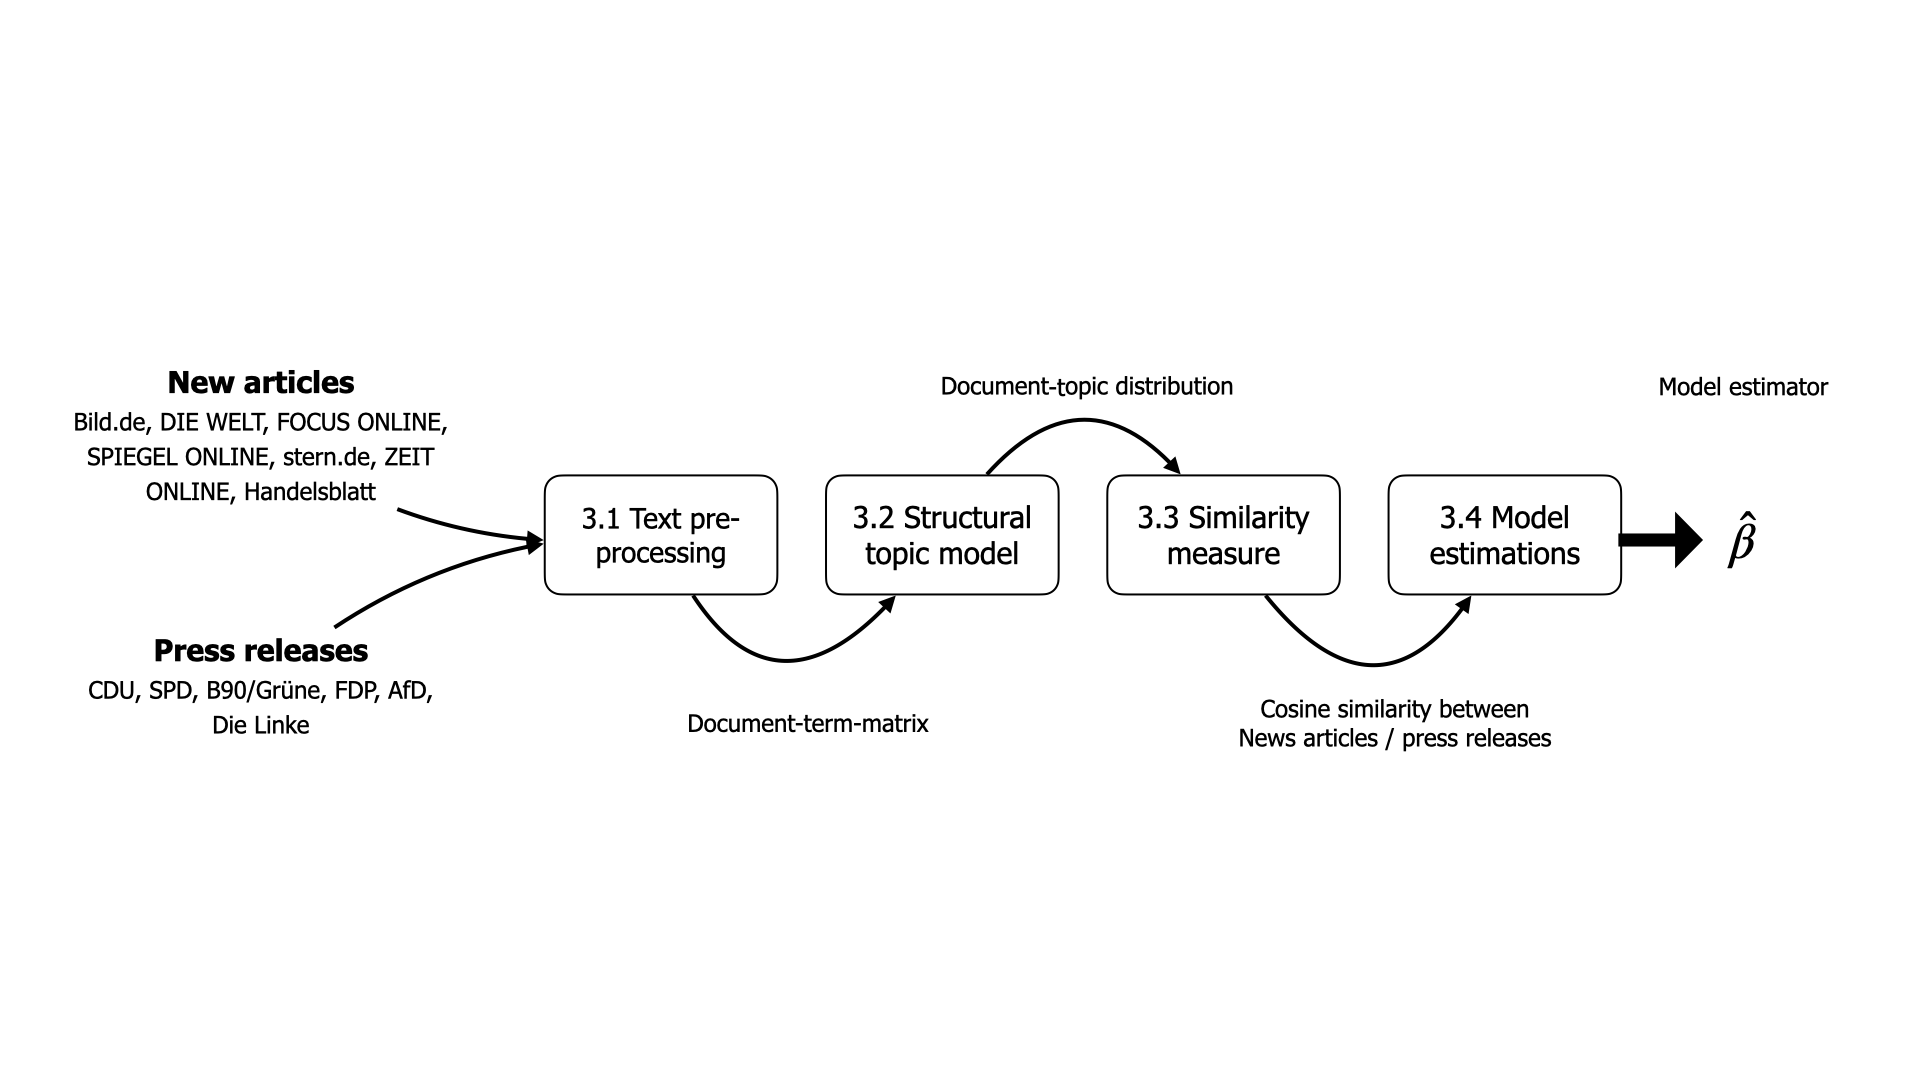
\includegraphics{../figs/high_level_overview.png}

\hypertarget{ii-background-information}{%
\section{II Background information}\label{ii-background-information}}

\hypertarget{the-political-situation-in-germany-june-2017---march-2018}{%
\subsection{The political situation in Germany (June 2017 - March
2018)}\label{the-political-situation-in-germany-june-2017---march-2018}}

The articles analyzed in this paper cover a period from June 1, 2017 to
March 1, 2018 and thus cover both the most important election campaign
topics for the Bundestag elections on September 24, 2017 and the process
of forming a government that lasted until February 2018. After four
years in a grand coalition with the Social Democrats (SPD), German
Chancellor Angela Merkel, member of the conservative party CDU/CSU (also
known as Union), ran for re-election. The SPD nominated Martin Schulz as
their candidate.

On the right side of the political spectrum, AfD (alternative for
Germany) managed to be elected to the German Bundestag for the first
time in 2017. The political debate about the high refugee numbers of the
past years brought a political upswing to the AfD, which used the
dissatisfaction of parts of the population to raise its own profile. In
the course of the reporting on the federal elections, leading party
members of the AfD as well as party supporters repeatedly accused the
mass media of reporting unilaterally and intentionally presenting the
AfD badly.

After the election, the formation of a government was difficult due to
the large number of parties elected to the Bundestag and the
considerable loss of votes by the major parties CDU/CSU and SPD. Since
all parties rejected a coalition with the AfD, numerically only two
coalitions with an absolute parliamentary majority were possible: a
grand coalition (``GroKo'' - from the German word Große Koalition) of
CDU/CSU and SPD, and a Jamaica coalition (coalition of CDU/CSU, FDP
(economic liberal party) and B90/Die Grünen (Bündnis 90/Die Grünen,
green party)). The grand coalition was initially rejected by the SPD.
The four-week exploratory talks on the possible formation of a Jamaica
coalition officially failed on November 19, 2017 after the FDP announced
its withdrawal from the negotiations. FDP party leader Christian Lindner
said that there had been no trust between the parties during the
negotiations. The main points of contention were climate and refugee
policy. CDU and CSU regretted this result, while B90/Die Grünen sharply
criticized the liberals' withdrawal. The then Green leader Cem Özdemir
accused the FDP of lacking the will to reach an agreement.

After the failure of the Jamaica coalition talks, a possible re-election
or a minority government as alternatives were discussed in the media
before the SPD decided to hold coalition talks with the CDU/CSU. This
led to great resistance from the party base, which called for a
party-internal referendum on a grand coalition. After the party members
voted in favor of the grand coalition, a government was formed 171 days
after the federal elections.

\autoref{fig:election_polls} shows that support for the two major
popular parties has been declining in recent months since August 2017,
with the CDU/CSU again showing positive survey results since November
2017.\footnote{For each party the survey results of the seven major
  institutes are considered. To calculate a smooth line for each party
  on each day, the moving average within 15 days (7 before the day, 7
  after the day, and the day itself) is estimated. The data source is
  \url{https://www.wahlrecht.de/}.} However,the poll results of the SPD
have been falling since March 2017. At the same time, the AfD in
particular has been recording increasingly positive survey results since
June 2017.

\begin{figure}

{\centering 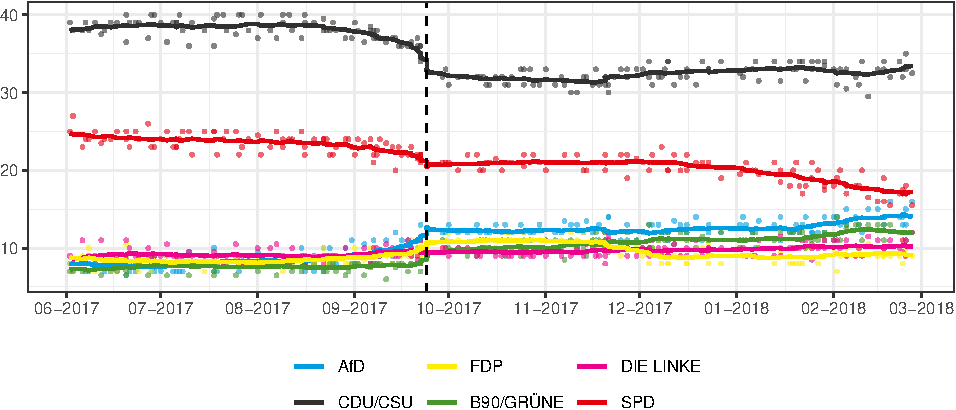
\includegraphics[width=0.5\linewidth]{main_text_files/figure-latex/election polls-1} 

}

\caption{Election polls during the period under review \label{fig:election_polls}}\label{fig:election polls}
\end{figure}

\hypertarget{german-online-news-market}{%
\subsection{German online news market}\label{german-online-news-market}}

The analysis performed in this paper is based on the news articles of
the following news websites: Bild.de, DIE WELT, FOCUS ONLINE,
Handelsblatt, SPIEGEL ONLINE, stern.de, ZEIT ONLINE. As can be seen from
\autoref{fig:news_market}(a), expect for Handelsblatt (position 53),
these media outlets are among the top 30 German online news providers in
the period under review in terms of visits.\footnote{The term visit is
  used to describe the call to a website by a visitor. The visit begins
  as soon as a user generates a page impression (PI) within an offer and
  each additional PI, which the user generates within the offer, belongs
  to this visit.}

The main source of income for these privately managed media houses is
digital advertising, even though paid content is playing an increasingly
important role. However, according to a survey on digital news by the
Reuters Institute (\protect\hyperlink{ref-newman_reuters_2018}{N. Newman
et al. 2018}) only 8\% of respondents pay for online news. The online
survey for German data was undertaken between 19th - 22nd January 2018
by the Hans Bredow Institute\footnote{\url{https://www.hans-bredow-institut.de/de/projekte/reuters-institute-digital-news-survey}}
with a total sample size of 2038 adults (aged 18+) who access news once
a month or more. Among other questions, participants were asked which
news sources they use to access news online.\footnote{The exact question
  was: ``Which of the following brands have you used to access news
  online in the last week (via websites, apps, social media, and other
  forms of Internet access)? Please select all that apply.''} The
results displayed in \autoref{fig:news_market}(b) indicate that the
media used for the analysis play a relevant role in their consumption.

\begin{figure}

{\centering \subfloat[Total visits in million (Jan 2018)\label{fig:unnamed-chunk-1-1}]{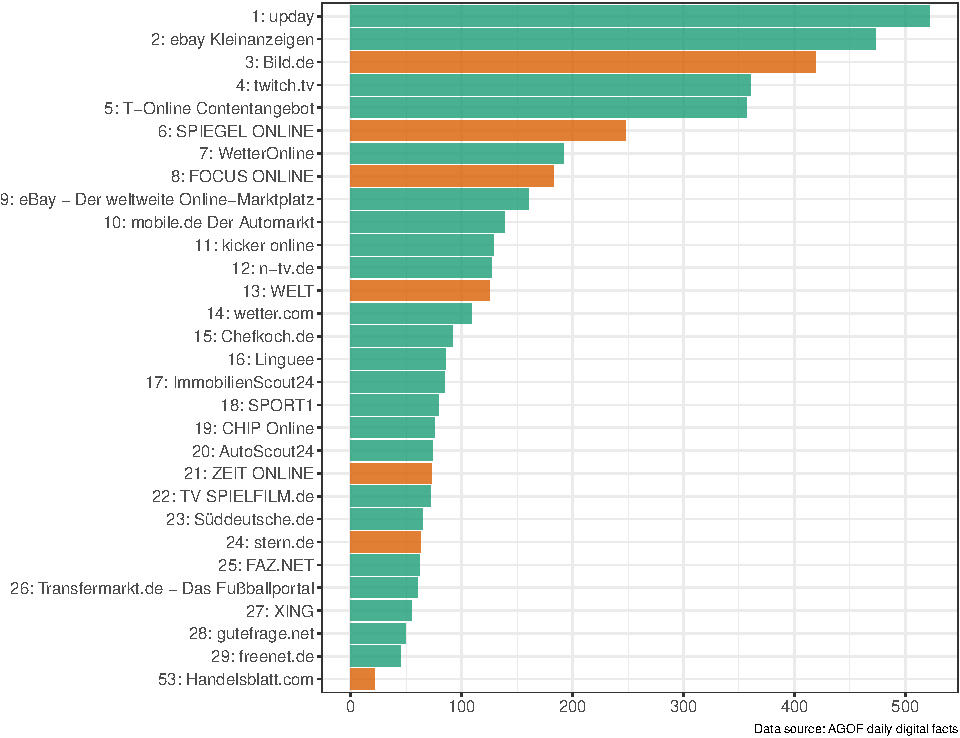
\includegraphics[width=0.4\linewidth]{main_text_files/figure-latex/unnamed-chunk-1-1} }\subfloat[Use of a brand to access news online\label{fig:unnamed-chunk-1-2}]{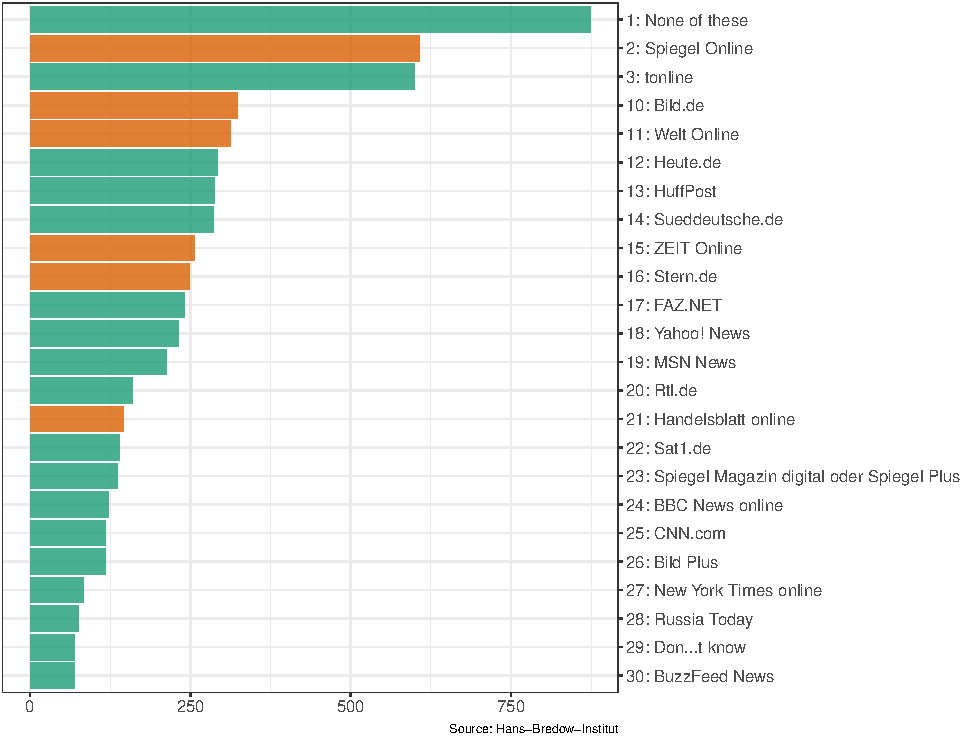
\includegraphics[width=0.4\linewidth]{main_text_files/figure-latex/unnamed-chunk-1-2} }

}

\caption{Selected german news brands \label{fig:news_market}}\label{fig:unnamed-chunk-1}
\end{figure}

\hypertarget{iii-text-data}{%
\section{III Text data}\label{iii-text-data}}

I conduct the estimation on a sample of 18,757 online news articles from
the seven German news providers described in the previous
section\footnote{Bild.de, DIE WELT, FOCUS ONLINE, SPIEGEL ONLINE,
  stern.de, ZEIT ONLINE, Handelsblatt} about domestic politics and press
releases of the seven parties that have been in the Bundestag since the
2017 federal elections\footnote{CDU, SPD, B90/Grüne, FDP, AfD, Die Linke}.
Both news articles and press releases are dated from June 1, 2017 to
March 1, 2018.

News articles scraped from the Webhose.io API.\footnote{For more
  information see
  \url{https://docs.webhose.io/reference\#about-webhose}.} In order to
consider only news about national politics, the articles were filtered
based on their URL. The press releases were scraped from the public
websites of the political parties and parliamentary groups using an
automated script.\footnote{The scraping code was written in R and can be
  made available on request.}

\autoref{fig:news_distr} shows the distribution of the number of
articles by date and media outlet. There is a high peak around the
federal elections on September, 24th and another one shortly after the
failure of the Jamaica coalition talks on November, 19th (indicated by
the red dotted lines).\footnote{The peak in July especially for stern.de
  is due to increased reporting about the G20 summit in Hamburg.}
Furthermore, \autoref{fig:news_distr} shows that DIE WELT published the
most articles on domestic policy, followed by stern.de, Handelsblatt and
FOCUS ONLINE.

\begin{figure}

{\centering 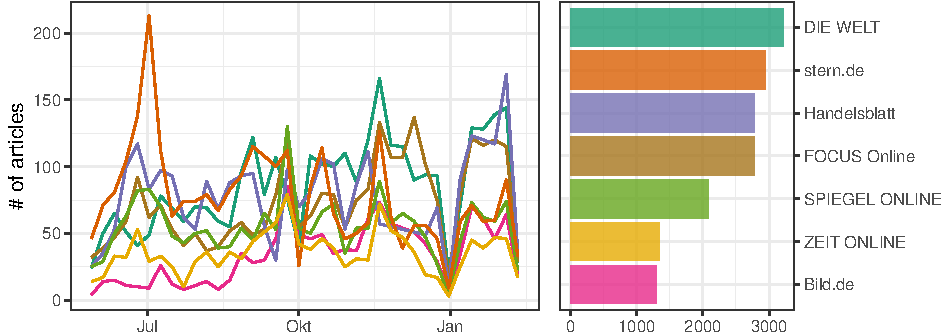
\includegraphics[width=0.7\linewidth]{main_text_files/figure-latex/Distribution of news articles-1} 

}

\caption{Distribution of news articles \label{fig:news_distr}}\label{fig:Distribution of news articles}
\end{figure}

\begin{figure}

{\centering 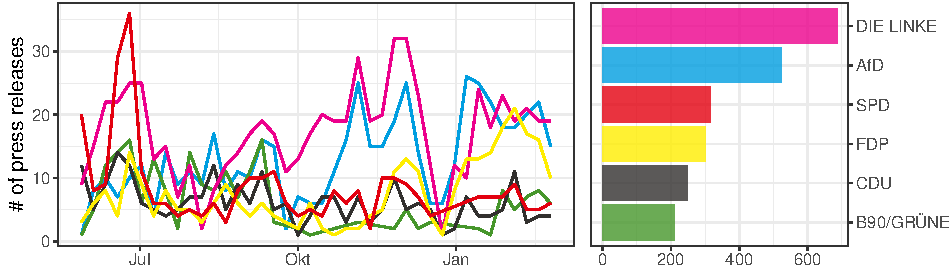
\includegraphics[width=0.7\linewidth]{main_text_files/figure-latex/Distribution of press releases-1} 

}

\caption{Distribution of press releases \label{fig:press_distr}}\label{fig:Distribution of press releases}
\end{figure}

\begin{table}[H]

\caption{\label{tab:table text length}Summary statistics of text length \label{tab:textlength}}
\centering
\fontsize{7}{9}\selectfont
\begin{tabular}[t]{lrrrrrr}
\toprule
source & n & mean & sd & median & min & max\\
\midrule
\addlinespace[0.3em]
\multicolumn{7}{l}{\textbf{News articles}}\\
\hspace{1em}\cellcolor{gray!6}{Bild.de} & \cellcolor{gray!6}{1303} & \cellcolor{gray!6}{476.07} & \cellcolor{gray!6}{318.28} & \cellcolor{gray!6}{398.0} & \cellcolor{gray!6}{121} & \cellcolor{gray!6}{3710}\\
\hspace{1em}DIE WELT & 3222 & 509.57 & 612.06 & 380.0 & 121 & 14507\\
\hspace{1em}\cellcolor{gray!6}{FOCUS Online} & \cellcolor{gray!6}{2780} & \cellcolor{gray!6}{393.89} & \cellcolor{gray!6}{317.05} & \cellcolor{gray!6}{297.5} & \cellcolor{gray!6}{121} & \cellcolor{gray!6}{5647}\\
\hspace{1em}Handelsblatt & 2785 & 589.51 & 495.82 & 488.0 & 121 & 6899\\
\hspace{1em}\cellcolor{gray!6}{SPIEGEL ONLINE} & \cellcolor{gray!6}{2089} & \cellcolor{gray!6}{539.09} & \cellcolor{gray!6}{415.05} & \cellcolor{gray!6}{413.0} & \cellcolor{gray!6}{121} & \cellcolor{gray!6}{3466}\\
\hspace{1em}stern.de & 2943 & 514.66 & 616.55 & 373.0 & 121 & 9287\\
\hspace{1em}\cellcolor{gray!6}{ZEIT ONLINE} & \cellcolor{gray!6}{1351} & \cellcolor{gray!6}{513.75} & \cellcolor{gray!6}{387.14} & \cellcolor{gray!6}{459.0} & \cellcolor{gray!6}{121} & \cellcolor{gray!6}{8015}\\
\addlinespace[0.3em]
\multicolumn{7}{l}{\textbf{Press releases}}\\
\hspace{1em}AfD & 523 & 212.83 & 72.16 & 196.0 & 103 & 553\\
\hspace{1em}\cellcolor{gray!6}{B90/GRÜNE} & \cellcolor{gray!6}{211} & \cellcolor{gray!6}{229.32} & \cellcolor{gray!6}{63.37} & \cellcolor{gray!6}{219.0} & \cellcolor{gray!6}{104} & \cellcolor{gray!6}{399}\\
\hspace{1em}CDU & 248 & 274.54 & 106.08 & 256.0 & 100 & 1030\\
\hspace{1em}\cellcolor{gray!6}{DIE LINKE} & \cellcolor{gray!6}{686} & \cellcolor{gray!6}{200.47} & \cellcolor{gray!6}{71.78} & \cellcolor{gray!6}{190.0} & \cellcolor{gray!6}{101} & \cellcolor{gray!6}{1048}\\
\hspace{1em}FDP & 301 & 161.90 & 83.78 & 144.0 & 100 & 999\\
\hspace{1em}\cellcolor{gray!6}{SPD} & \cellcolor{gray!6}{315} & \cellcolor{gray!6}{213.41} & \cellcolor{gray!6}{56.16} & \cellcolor{gray!6}{208.0} & \cellcolor{gray!6}{103} & \cellcolor{gray!6}{429}\\
\bottomrule
\end{tabular}
\end{table}

\autoref{tab:textlength} illustrates that on average, news articles are
longer than the parties' press releases.\footnote{News articles with
  less than 120 words were filtered out in advance, as these were mostly
  reader comments. Similarly press releases with less than 100 words
  were filtered out.} While for news articles the average is between 394
(FOCUS Online) and 590 (Handelsblatt), with press releases the range is
between 162 (FDP) and 275 (CDU). The article with the most words
(14.507) was published by DIE WELT - the longest press release has 1.048
words and was published by DIE LINKE.

\hypertarget{text-pre-processing}{%
\subsection{Text pre-processing}\label{text-pre-processing}}

To use text as data for statistical analysis, different pre-processing
steps have to be conducted. In fact, in order to use text as data and
reduce the dimensionality to avoid unnecessary computational complexity
and overfitting, pre-processsing the text is a central task in text
mining (\protect\hyperlink{ref-gentzkow_text_2017}{M. Gentzkow, Kelly,
and Taddy} (\protect\hyperlink{ref-gentzkow_text_2017}{2017}),
\protect\hyperlink{ref-bholat_text_2015}{Bholat et al.}
(\protect\hyperlink{ref-bholat_text_2015}{2015})). Intuitively the term
frequency (tf) of a word is a measure of how important that word may be
for the understanding of the text. To visualize these terms, word clouds
are a commonly used technique in text mining as they translate the tf
into the size of the term in the cloud. As can be seen in
\autoref{fig:wordcloud1}, problems arise with words that are highly
frequent. For example ``die,'' or ``der'' (eng. ``the''), ``und'' (eng.
``and''), and ``ist'' (eng. ``is'') are extremely common but unrelated
to the quantity of interest. These terms, often called stop words
(\protect\hyperlink{ref-gentzkow_text_2017}{M. Gentzkow, Kelly, and
Taddy 2017}), are important to the grammatical structure of a text, but
typically don't add any additional meaning and can therefore be
neglected.

\begin{figure}

{\centering 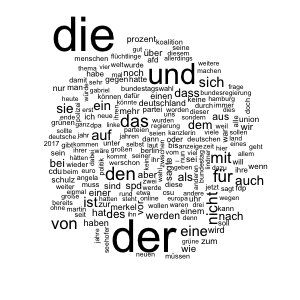
\includegraphics[width=0.4\linewidth]{../figs/wordcloud} 

}

\caption{Wordcloud before pre-processing \label{fig:wordcloud1}}\label{fig:wordcloud pre-processing}
\end{figure}

To remove distorting words, the pre-defined stop word list from the
Snowball project\footnote{\url{http://snowball.tartarus.org/algorithms/german/stop.txt}}
is used together with a customized, domain-specific list of stop-words.
Additionally punctuation character (e.g.~., ,, !, ?, etc.) and all
numbers are removed from the data. A next step to reduce the
dimensionality of text data is to apply an adequate stemming technique.
Stemming is a process by which different morphological variants of a
word are traced back to their common root. For example, ``voting'' and
``vote'' would be treated as two instances of the same token after the
stemming process. There are many different techniques for the stemming
process. I apply the widely used Porter-Stemmer algorithm, which is
based on a set of shortening rules that are applied to a word until it
has a minimum number of syllables.\footnote{\url{https://tartarus.org/martin/PorterStemmer/}}

As an example, the following word clouds represent the most frequent
words of the pre-processed articles for Bild.de
(\autoref{fig:wordclouds2}(a)) and press releases of AfD
(\autoref{fig:wordclouds2}(b)). It becomes evident that these are texts
discussing domestic policy issues. The SPD in particular seems to be
highly frequent for Bild.de.

\begin{figure}

{\centering \subfloat[Bild\label{fig:wordclouds2-1}]{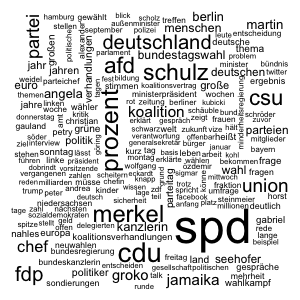
\includegraphics[width=0.4\linewidth]{../figs/wordcloud_bild} }\subfloat[AfD\label{fig:wordclouds2-2}]{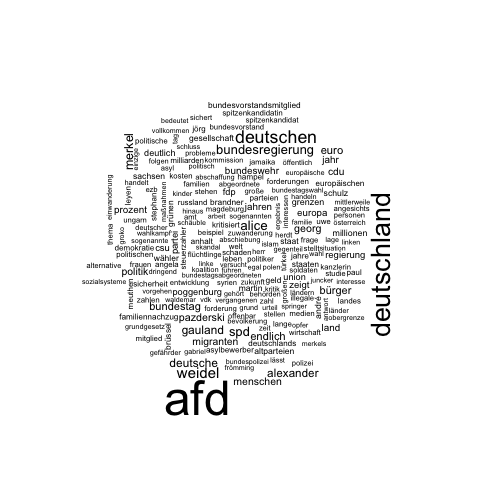
\includegraphics[width=0.4\linewidth]{../figs/wordcloud_afd} }

}

\caption{Wordcloud after pre-processing \label{fig:wordclouds2}}\label{fig:wordclouds2}
\end{figure}

The next step is to divide the entire data set into individual documents
and to represent these documents as a finite list of unique terms. In
this setting, each news article and each press release represents a
document \(d\), whereby each of these documents can be assigned to a
news website or a party. The sum of all documents forms what is called
the corpus. For each document \(d \in \lbrace 1,...,D \rbrace\) the
number of occurrences of term \(v\) in document \(d\) is computed, in
order to obtain the count \(x_{d,v}\), where each unique term in the
corpus is indexed by some \(v \in \lbrace 1,...,V \rbrace\) and where
\(V\) is the number of unique terms. The \(D\) x \(V\) matrix
\(\boldsymbol{X}\) of all such counts is called the document-term
matrix. Each row in this matrix represents a document, where each entry
in this row counts the occurrences of a unique term in that document.
\autoref{table:dtm} provides a sample output of the document-term matrix
used in this paper, where each document is represented by a unique id
(the row name in the example below). This representation is often
referred to as the bag of words model
(\protect\hyperlink{ref-gentzkow_text_2017}{M. Gentzkow, Kelly, and
Taddy 2017}), since the order in which words are used within a document
is disregarded.

\begin{table}[H]

\caption{\label{tab:Document term matrix}Document-term matrix - sample values \label{table:dtm}}
\centering
\fontsize{7}{9}\selectfont
\begin{tabular}[t]{lrrrrrrr}
\toprule
  & lkw & vorläufigen & bringe & streit & meldung & vermitteln & bundestagspräsidenten\\
\midrule
\cellcolor{gray!6}{4553} & \cellcolor{gray!6}{0} & \cellcolor{gray!6}{0} & \cellcolor{gray!6}{0} & \cellcolor{gray!6}{0} & \cellcolor{gray!6}{0} & \cellcolor{gray!6}{0} & \cellcolor{gray!6}{0}\\
17827 & 0 & 0 & 0 & 0 & 0 & 0 & 0\\
\cellcolor{gray!6}{3523} & \cellcolor{gray!6}{0} & \cellcolor{gray!6}{0} & \cellcolor{gray!6}{0} & \cellcolor{gray!6}{0} & \cellcolor{gray!6}{0} & \cellcolor{gray!6}{0} & \cellcolor{gray!6}{0}\\
16982 & 0 & 0 & 0 & 0 & 0 & 0 & 0\\
\cellcolor{gray!6}{4051} & \cellcolor{gray!6}{0} & \cellcolor{gray!6}{0} & \cellcolor{gray!6}{0} & \cellcolor{gray!6}{0} & \cellcolor{gray!6}{0} & \cellcolor{gray!6}{0} & \cellcolor{gray!6}{0}\\
\addlinespace
4466 & 0 & 0 & 0 & 0 & 0 & 0 & 1\\
\cellcolor{gray!6}{15332} & \cellcolor{gray!6}{0} & \cellcolor{gray!6}{0} & \cellcolor{gray!6}{0} & \cellcolor{gray!6}{0} & \cellcolor{gray!6}{0} & \cellcolor{gray!6}{0} & \cellcolor{gray!6}{0}\\
1984 & 0 & 0 & 0 & 0 & 0 & 0 & 0\\
\cellcolor{gray!6}{11404} & \cellcolor{gray!6}{0} & \cellcolor{gray!6}{0} & \cellcolor{gray!6}{0} & \cellcolor{gray!6}{0} & \cellcolor{gray!6}{0} & \cellcolor{gray!6}{0} & \cellcolor{gray!6}{0}\\
7287 & 0 & 0 & 0 & 0 & 0 & 0 & 0\\
\bottomrule
\end{tabular}
\end{table}

\hypertarget{iv-estimate-topic-similarity-of-documents}{%
\section{IV Estimate topic similarity of
documents}\label{iv-estimate-topic-similarity-of-documents}}

\hypertarget{a-structural-topic-model-to-identify-the-latent-topics}{%
\subsection{A structural topic model to identify the latent
topics}\label{a-structural-topic-model-to-identify-the-latent-topics}}

To discover the latent topics in the corpus of press releases and news
articles, a structural topic modeling (STM) developed by
(\protect\hyperlink{ref-roberts_model_2016}{M. E. Roberts, Stewart, and
Airoldi 2016}) is applied. In general, topic models formalize the idea
that documents are formed by hidden variables (topics) that generate
correlations among observed terms. They belong to the group of
unsupervised generative models, meaning that the true attributes
(topics) cannot be observed. The STM is an extension of the standard
topic modelling technique, labeled as latent Dirichlet allocation (LDA),
which refers to the Bayesian model in
\protect\hyperlink{ref-blei_latent_2003}{Blei, Ng, and Jordan}
(\protect\hyperlink{ref-blei_latent_2003}{2003}) that treats each word
in a topic and each topic in a document as generated from a
Dirichlet-distributed prior.\footnote{See also
  \protect\hyperlink{ref-griffiths_probabilistic_2002}{Griffiths and
  Steyvers}
  (\protect\hyperlink{ref-griffiths_probabilistic_2002}{2002}),
  \protect\hyperlink{ref-griffiths_finding_2004}{Griffiths and Steyvers}
  (\protect\hyperlink{ref-griffiths_finding_2004}{2004}) and
  \protect\hyperlink{ref-hofmann_probabilistic_1999}{Hofmann}
  (\protect\hyperlink{ref-hofmann_probabilistic_1999}{1999})}.

The underlying idea for these models suggests that each individual topic
\(k\) potentially contains all of the unique terms within the vocabulary
\(V\) with different probability. Therefore, each topic \(k\) can be
represented as a probability vector \(\phi_k\) over all unique terms
\(V\). Simultaneously, each individual document \(d\) in the corpus can
be represented as a probability distribution \(\theta_d\) over the \(K\)
topics.

The STM is an extension of the LDA process since it allows covariates of
interest (such as the publication date of a document or it's author) to
be included in the prior distributions for both topic proportions
(\(\theta\)) and topic-word distributions (\(\phi\)). This way, STM
offers a method of `structuring' the prior distributions in the topic
model, including additional information in the statistical inference
procedure, while LDA assumes that \(\theta ~ \text{Dirichlet}(\alpha)\)
and \(\phi ~ \text{Dirichlet}(\beta)\), where \(\alpha\) and \(\beta\)
are fitted with the model.

In order to include the covariates in the statistical inference
procedure, two design matrices of covariates (\(X\) and \(Z\)) are
specified, where each row defines a vector of covariates for a specific
document. In \(X\), the covariates for topic prevalence are given, so
that the probability of a topic for each document varies according to
\(X\), rather than resulting from a single common prior. The same
applies to \(Z\), in which the covariates for the word distribution
within a topic are specified. The underlying data generating process to
generate each individual word \(w_{d,n}\) in a document \(d\) for the
\(n^{th}\) word-position can be described as follows:

\begin{itemize}
\tightlist
\item
  for each document \(i\), draw its distribution of topics \(\theta_d\)
  depending on the metadata included in the model defined in \(X\);
\item
  for each topic \(k\), draw its distribution of words \(\phi_k\)
  depending on the metadata included in the model defined in \(Z\);
\item
  for each word \(n\), draw its topic \(z_n\) based on \(\theta_i\);
\item
  for each word word \(n\), draw the term distribution for the selected
  topic \(\phi_{z_{d,n}}\).
\end{itemize}

One crucial assumption to be made for topic models like LDA or STM is
the number of topics (\(K\)) that occur over the entire corpus. There is
not a ``right'' answer to the number of topics that are appropriate for
a given corpus (\protect\hyperlink{ref-grimmer_text_2013}{Grimmer and
Stewart 2013}). \protect\hyperlink{ref-roberts_stm:_2016}{M. Roberts,
Stewart, and Tingley} (\protect\hyperlink{ref-roberts_stm:_2016}{2016b})
propose to measure topic quality through a combination of semantic
coherence and exclusivity of words to topics. Semantic coherence is a
criterion developed by
\protect\hyperlink{ref-mimno_optimizing_2011}{Mimno et al.}
(\protect\hyperlink{ref-mimno_optimizing_2011}{2011}) and is closely
related to pointwise mutual information
(\protect\hyperlink{ref-newman_automatic_2010}{D. Newman et al. 2010}):
it is maximized when the most probable words in a given topic frequently
co-occur together.

Using the function \(searchK\) from the \(stm\) package several
automated tests are performed to help choose the number of topics
including the average exclusivity and semantic coherence as well as the
held out likelihood
(\protect\hyperlink{ref-wallach_rethinking_2009}{Wallach, Mimno, and
McCallum 2009}) and the residuals
(\protect\hyperlink{ref-taddy_estimation_2012}{Taddy 2012}). This
process revealed that a model with 40 topics best reflects the structure
in the corpus. Furthermore, I use the author and bi-week dummies of a
document as topical prevalence variable. In other words, I assume that
the probability of a topic to be included in a news article or a press
release depends on the author of that document and when it was
published. I argue that these variables are best suited to capture
temporal and publisher level variation in the documents.

\begin{verbatim}
## stm(documents = news_df_sparse, K = 40, prevalence = ~source + 
##     s(year_biweek), data = covariates, init.type = "Spectral")
\end{verbatim}

In general inference of mixed-membership models, such as the one applied
in this paper, has been a thread of research in applied statistics
\protect\hyperlink{ref-braun_variational_2010}{Braun and McAuliffe}
(\protect\hyperlink{ref-braun_variational_2010}{2010}). Topic models are
usually imprecise as the function to be optimized has multiple modes,
such that the model results can be sensitive to the starting values
(e.g.~the number of topics and the covariates influencing the prior
distributions). Since an ex ante valuation of a model is hardly
possible, I compute a variety of different models and compare their
posterior probability. This enables me to check how results vary for
different model specifications
(\protect\hyperlink{ref-roberts_navigating_2016}{M. Roberts, Stewart,
and Tingley 2016a}). I then cross-checked some subset of assigned topic
distributions to evaluate whether the estimates align with the concept
of interest (\protect\hyperlink{ref-gentzkow_text_2017}{M. Gentzkow,
Kelly, and Taddy 2017}).

\hypertarget{results-of-the-stm}{%
\subsection{Results of the STM}\label{results-of-the-stm}}

As mentioned in the previous section, the generative process of the STM
results in a topic distribution \(\theta_d\) for each document \(d\)
over all topics \(k\) and a word distribution \(\phi_k\) for each topic
over all terms in the vocabulary. The most probable words of each topic
may help to understand what each topic is about.\footnote{\autoref{table:top_terms}
  gives an overview of the most probable terms for each topic.} However,
since those most probable words are not necessarily the most exclusive
words and they only represent a small fraction of the probability
distribution, interpretation should be done very cautiously.

For our analysis, we use the topic distribution of each document to
estimate the similarity of documents. \autoref{fig:sample_docs12}
illustrates such a topic distribution of two news paper articles. The
red numbers display the topic probability (for probabilities
\(>= 0.02\)). News article 1\footnote{Bundeswehr scandal: ex-commander
  attacks Von Der Leyen} shows a clear distribution towards topic 36,
for which terms like Bundeswehr, Soldaten (soldiers), Nato,
Verteidigungsministerin (defense minister) are among the most probable
words. News article 2\footnote{Bundestag elections: 42 parties want to
  be elected to parliament.} does not show such a clear tendency towards
a single topic. Topic 40, 18 and 5 are within a comparable range.
However, for all three topics similar terms are among the top terms.

Similarly as for the news articles, \autoref{fig:sample_docs34}
illustrates the topic distribution for two press releases randomly
chosen from the corpus. For press release 1\footnote{Lars Herrmann: The
  danger for Germany and its Basic Law is also coming from the left}
topic 24 is the most probable topic which contains terms about the G20
Summit, during which left-wing radicals caused considerable riots. Topic
distribution of press article 2\footnote{Trump chooses the path to
  isolation} shows peaks for topic 6 and 35. Top terms of topic 6
contain the words trump, us, usa, deutschland (Germany) and präsident
(president). Similarly topic 35 seems to deal with German foreign
policy, since top terms include words like eu, deutschland (Germany),
europa and bundesregierung (Federal Government).

\begin{figure}

{\centering 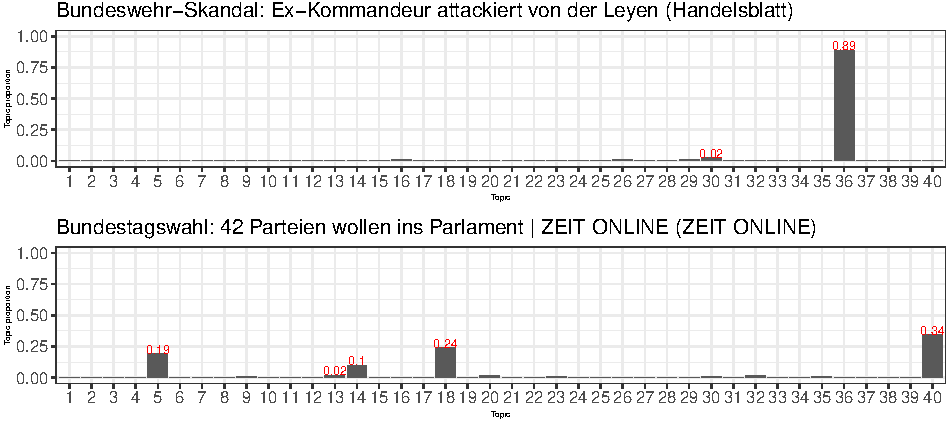
\includegraphics[width=0.8\linewidth]{main_text_files/figure-latex/News articles sample documents-1} 

}

\caption{Topic probability of sample news articles \label{fig:sample_docs12}}\label{fig:News articles sample documents}
\end{figure}

\begin{figure}

{\centering 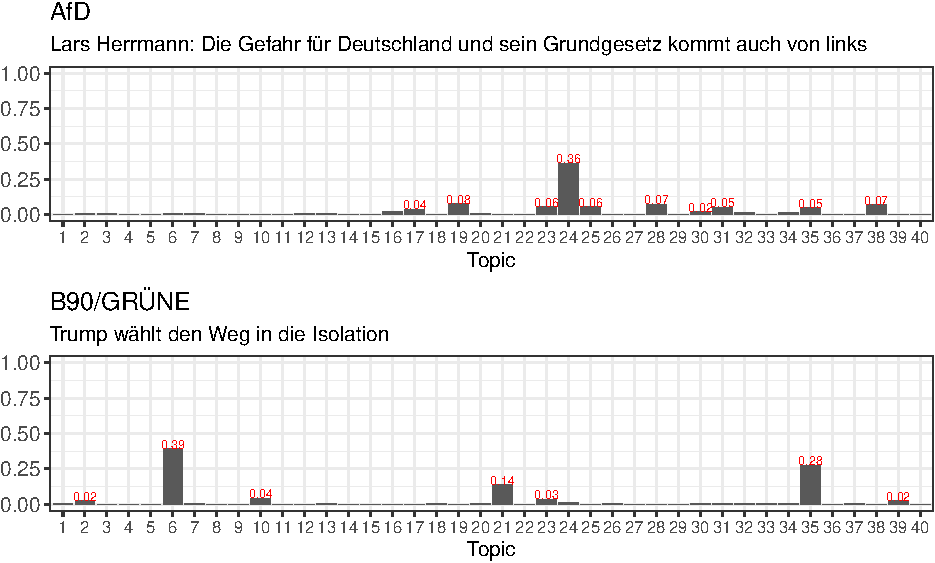
\includegraphics[width=0.8\linewidth]{main_text_files/figure-latex/Press releases sample documents-1} 

}

\caption{Topic probability of sample press releases \label{fig:sample_docs34}}\label{fig:Press releases sample documents}
\end{figure}

Since the source and publication date is known for each document, the
probability of certain topics can be analysed, aggregated by this
metadata. The left chart of \autoref{fig:sample_topics_afd} is showing
the 15 topics with the highest probability for press releases published
by the AfD. The right side of the figure is aggregating the probability
by source and time (in weeks) for two sample topics, displaying how they
change over time in the AfD press releases compared to two sample news
papers. It becomes clear, that topic 9\footnote{translation: afd, party,
  saxony, gauland, parties, pazderski, höcke} is systematically more
likely in the AfD's press releases compared to the two newspapers. There
is a noticeable increase in probability during the election campaign
period and ends in a peak on election day itself. For Handelsblatt and
Bild.de, too, a slight increase around election day is discernible and
the probability of this topic shows some peaks for Bild.de both before
and after the election. The top words of Theme 38\footnote{translation:
  refugees, germany, people, number, refugees, family reunion, year}
suggest that it addresses refugees - a topic the AfD has a very clear
position on. The probability of this topic increases in the AfD's press
releases until about a month before the election and then levels off
somewhat. A similar trend can be seen for the news articles from
Bild.de. The curve from Handelsblatt is rather flat and shows no
apparent difference between before and after the election.

\begin{figure}

{\centering 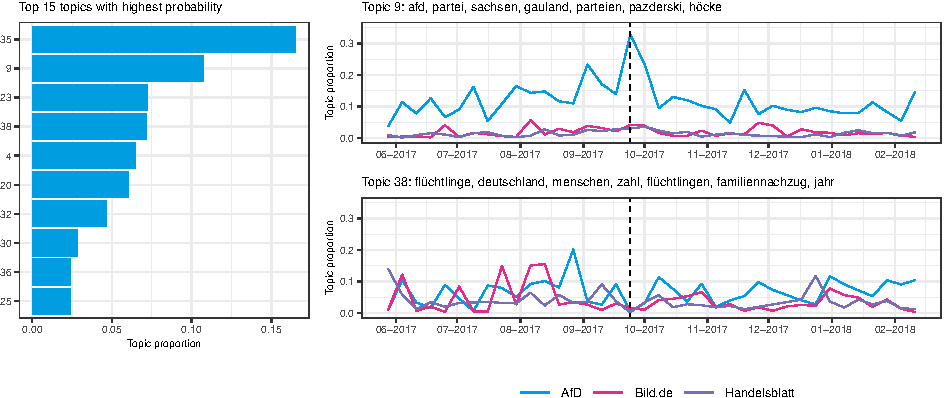
\includegraphics[width=1\linewidth]{main_text_files/figure-latex/Top AfD topics-1} 

}

\caption{Comparison of topic probability - sample topics AfD \label{fig:sample_topics_afd}}\label{fig:Top AfD topics}
\end{figure}

\autoref{fig:sample_topics_fdp} is doing a similar analysis for the
aggregated topic distribution in press releases of the FDP. The chart on
the left illustrates that, as in the case of the AfD, the topic 35 has
the highest probability in the press releases of the FDP. Unlike in the
case of the AfD, however, this is followed by topics that have clearer
temporal peaks, as shown on the right using two example topics. Topic
10\footnote{translation: diesel, enterprises, germany, cars, german,
  industry, driving bans} has a clear peak for both the news papers and
the FDP press releases around august 2017. At that time, there was a
debate about whether and where driving bans for diesel cars would be
introduced. After the states of Baden-Württemberg and North
Rhine-Westphalia initially filed a lawsuit against this, the court
proceedings that would decide whether driving bans are permissible began
in mid-February 2018. The temporal curve of the FDP shows a further
increase in topic probability at this time, which can also be detected
at Handelsblatt. At Bild.de, however, the topic is apparently only taken
up once briefly in August 2017, as only a very low topic probability can
be seen thereafter. The peak of the probabilty of topic 39\footnote{translation:
  fdp, grünen, jamaika, cdu, union, grüne, cdu} in all three sources
right after the election is reflecting the exploratory talks on the
possible formation of a Jamaica coalition, which officially failed on
November 19, 2017 after the FDP announced its withdrawal from the
negotiations.

\begin{figure}

{\centering 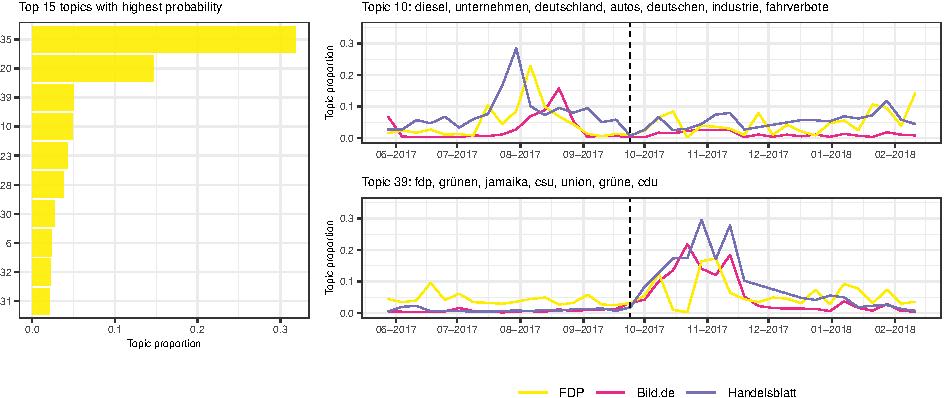
\includegraphics[width=1\linewidth]{main_text_files/figure-latex/Top FDP topics-1} 

}

\caption{Comparison of topic probability - sample topics FDP \label{fig:sample_topics_fdp}}\label{fig:Top FDP topics}
\end{figure}

\hypertarget{cosine-similarity}{%
\subsection{Cosine similarity}\label{cosine-similarity}}

Next, the cosine similarity measure is used in order to compare the
retrieved topic distribution of documents. Cosine similarity is a
measure for the distance between two vectors and is defined between zero
and one; values towards 1 indicate similarity. As topic proportions per
document are vectors of the same length, the cosine similarity allows a
comparison of the topic distribution between two documents.\footnote{For
  applications of cosine similarity to compare of topic model outcomes
  see e.g. \protect\hyperlink{ref-rehs_structural_2020}{Rehs}
  (\protect\hyperlink{ref-rehs_structural_2020}{2020}) and
  \protect\hyperlink{ref-ramage_characterizing_2010}{Ramage, Dumais, and
  Liebling} (\protect\hyperlink{ref-ramage_characterizing_2010}{2010})}

\[
\text{CS} = \text{cos}(\theta)=\frac{a*b}{||a|| ||b||}
\]

For example, \autoref{table:cosine_sim_sample_doc}\footnote{Translations:
  1) Asylum figures 2017 - black-red (synonym for GroKo) introduces
  upper limit through the back door (DIE LINKE) 2) Jörg Meuthen: Not a
  new GroKo, but LoKo - Loser Coalition (AfD) 3) Pension plans of Union
  and SPD worse than expected (FDP) 4) Union and SPD stabilize the
  extreme social injustice in this country (DIE LINKE) 5) Jürgen Pohl:
  Union and SPD agree on policy at the expense of pensioners and East
  Germans (AfD)} displays the most similar documents of the document
with the title \emph{Parteitag, Koalitions-Krimi, Ur-Wahl - Woran kann
die GroKo jetzt noch scheitern? (Bild.de)}.\footnote{Translation: Party
  conference, coalition thriller, primal election - what can fail the
  GroKo now? (Bild.de)}

\begin{table}[H]

\caption{\label{tab:Documents with highest similarity}Most similar documents \label{table:cosine_sim_sample_doc}}
\centering
\fontsize{7}{9}\selectfont
\begin{tabular}[t]{llr}
\toprule
title & source & cos\_sim\\
\midrule
\cellcolor{gray!6}{Asylzahlen 2017 - schwarz-rot führt Obergrenze durch die Hintertür ein} & \cellcolor{gray!6}{DIE LINKE} & \cellcolor{gray!6}{0.542}\\
Jörg Meuthen: Nicht neue GroKo, sondern LoKo – Loser Koalition & AfD & 0.522\\
\cellcolor{gray!6}{Rentenpläne von Union und SPD schlimmer als erwartet} & \cellcolor{gray!6}{FDP} & \cellcolor{gray!6}{0.478}\\
Union und SPD stabilisieren die krasse soziale Ungerechtigkeit in diesem Land & DIE LINKE & 0.401\\
\cellcolor{gray!6}{Jürgen Pohl: Union und SPD verabreden Politik zu Lasten von Rentnern und Ostdeutschen} & \cellcolor{gray!6}{AfD} & \cellcolor{gray!6}{0.388}\\
\bottomrule
\end{tabular}
\end{table}

In the next step, for each news paper, the cosine similarity between all
topic-document distribution pairs between the news papers articles and
the press releases is calculated if that press releases was published
within 7 days before the publication date of the news article. This
means the topic distribution of news article 1 is compared to press
release 1, 2, 3 and so on as long as the press release was published
within 7 days before the news article.
\autoref{table:dataset_structure1} illustrates a sample subset of the
data for DIE WELT.

\begin{table}[H]

\caption{\label{tab:Dataset structure 1}Dataset structure step 1 - DIE WELT \label{table:dataset_structure1}}
\centering
\fontsize{7}{9}\selectfont
\begin{tabular}[t]{llrllll}
\toprule
title1 & title2 & cosine\_sim & source1 & source2 & date1 & date2\\
\midrule
\cellcolor{gray!6}{Bundestagswahl 20...} & \cellcolor{gray!6}{Georg Pazderski: ...} & \cellcolor{gray!6}{0.04} & \cellcolor{gray!6}{DIE WELT} & \cellcolor{gray!6}{AfD} & \cellcolor{gray!6}{2018-01-26} & \cellcolor{gray!6}{2018-01-26}\\
SPD-Kritik an Mer... & Alice Weidel: Imm... & 0.02 & DIE WELT & AfD & 2017-11-28 & 2017-11-28\\
\cellcolor{gray!6}{Kooperationsverbo...} & \cellcolor{gray!6}{Götz Frömming:  U...} & \cellcolor{gray!6}{0.47} & \cellcolor{gray!6}{DIE WELT} & \cellcolor{gray!6}{AfD} & \cellcolor{gray!6}{2018-02-02} & \cellcolor{gray!6}{2018-01-29}\\
RCDS-Vorsitzender... & JEFTA: Zurück in ... & 0.22 & DIE WELT & B90/GRÜNE & 2017-07-11 & 2017-07-06\\
\cellcolor{gray!6}{Jeder zweite Deut...} & \cellcolor{gray!6}{DIE LINKE fordert...} & \cellcolor{gray!6}{0.01} & \cellcolor{gray!6}{DIE WELT} & \cellcolor{gray!6}{DIE LINKE} & \cellcolor{gray!6}{2017-06-07} & \cellcolor{gray!6}{2017-06-02}\\
\bottomrule
\end{tabular}
\end{table}

Next, the mean cosine similarity for each news article publication date
(date1) and party (source2) is estimated to obtain the final data frame
(see \autoref{table:dataset_structure_final}).

\begin{table}[H]

\caption{\label{tab:Dataset structure final}Final dataset structure - DIE WELT \label{table:dataset_structure_final}}
\centering
\fontsize{7}{9}\selectfont
\begin{tabular}[t]{lllr}
\toprule
date1 & source1 & source2 & cos\_sim\\
\midrule
\cellcolor{gray!6}{2017-12-04} & \cellcolor{gray!6}{DIE WELT} & \cellcolor{gray!6}{DIE LINKE} & \cellcolor{gray!6}{0.09}\\
2017-06-16 & DIE WELT & SPD & 0.19\\
\cellcolor{gray!6}{2018-01-15} & \cellcolor{gray!6}{DIE WELT} & \cellcolor{gray!6}{AfD} & \cellcolor{gray!6}{0.20}\\
2017-07-30 & DIE WELT & B90/GRÜNE & 0.13\\
\cellcolor{gray!6}{2017-09-26} & \cellcolor{gray!6}{DIE WELT} & \cellcolor{gray!6}{CDU} & \cellcolor{gray!6}{0.07}\\
\bottomrule
\end{tabular}
\end{table}

\hypertarget{v-model-estimations}{%
\section{V Model estimations}\label{v-model-estimations}}

To get a first idea of the trend of the data over time, the mean cosine
similarity between the news articles and each parties press releases
conditional on the day can be plotted.
\autoref{fig:mean_cosine_sim_ols_example} shows that kind of plot for
Handelsblatt and Bild.de (See \autoref{fig:mean_cosine_sim_ols} for all
news papers). Based on these figures, a few observations can be made.
The similarity with the FDP, e.g., seems to increase over time for both
Handelsblatt and Bild.de. In the case of Bild.de, this applies to all
parties, except for the AfD, where a slight downward trend is
discernible.

\begin{figure}

{\centering 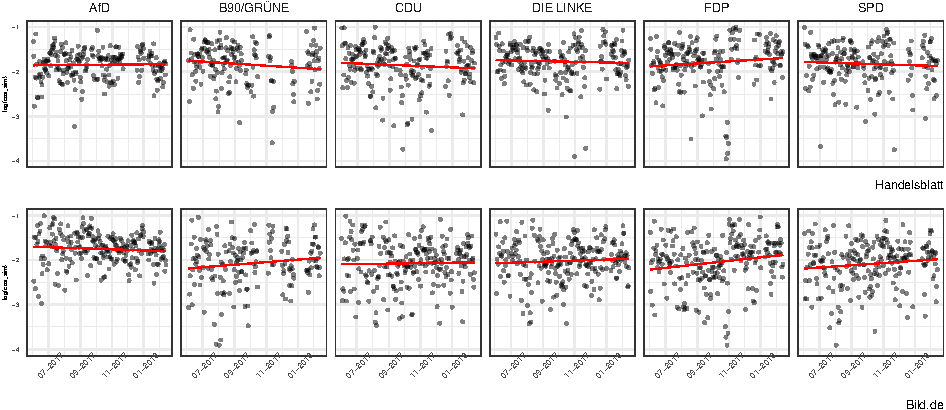
\includegraphics[width=0.9\linewidth]{main_text_files/figure-latex/Daily mean cosine similarity - example-1} 

}

\caption{Log of daily mean cosine similarity between newspaper/press articles pairs \label{fig:mean_cosine_sim_ols_example}}\label{fig:Daily mean cosine similarity - example}
\end{figure}

\hypertarget{ols-dummy-regression}{%
\subsection{OLS dummy regression}\label{ols-dummy-regression}}

To measure whether there is a significant difference in the topic
similarity for each party for a news publisher, a simple OLS regression
is estimated, where the similarity score (\(\ln(\text{CS}_{i})\)) on day
\(i\) between the news articles of that news publisher and the press
releases of a political party \(k\) is the dependent variable and the
political party dummies are the independent variables.

\[
\ln(\text{CS}_{t})=\beta_0+\beta_nD_{t,k-1}+\epsilon_t\text{,}
\]

with \(t\) = date\footnote{date1 in
  \autoref{table:dataset_structure_final}}, \(k\) = political
party\footnote{source2 in \autoref{table:dataset_structure_final}}

\autoref{table:results_ols} display the result of that estimation. Since
the dependent variable is log transformed, the the \% impact of \(D\) on
\(Y\) can be estimated as \(exp(\beta)-1\). E.g. since the transformed
coefficient for \(D_{B90/GRÜNE}\) is \(-0.2067\), a switch from from 0
to 1 can be interpreted as a 21\% decrease of topic similarity for
B90/GRÜNE compared to AfD (the base dummy group), holding everything
else equal. Or, in other words: Compared to AfD, the similarity of
topics of DIE WELT and B90/GRÜNE is 21\% lower. In general, for all news
papers (except for Handelsblat) the topic similarity is significantly
less between the news articles of that news paper and press releases of
political parties when compared to press releases of the AfD.

\begin{table}[!htbp] \centering    \caption{Results from the OLS model}    \label{table:results_ols}  \resizebox{0.99\textwidth}{!}{\begin{tabular}{@{\extracolsep{5pt}}lccccccc}  \\[-1.8ex]\hline  \hline \\[-1.8ex]   & \multicolumn{7}{c}{\textit{Dependent variable:}} \\  \cline{2-8}  \\[-1.8ex] & \multicolumn{7}{c}{Cosine similarity of topic distribution} \\   & DIE WELT & stern.de & ZEIT ONLINE & Handelsblatt & FOCUS Online & Bild.de & SPIEGEL ONLINE \\  \\[-1.8ex] & (1) & (2) & (3) & (4) & (5) & (6) & (7)\\  \hline \\[-1.8ex]   source2B90/GRÜNE & $-$0.232$^{***}$ & $-$0.237$^{***}$ & $-$0.220$^{***}$ & 0.033 & $-$0.297$^{***}$ & $-$0.319$^{***}$ & $-$0.202$^{***}$ \\    & (0.036) & (0.045) & (0.057) & (0.050) & (0.038) & (0.055) & (0.045) \\    & & & & & & & \\   source2CDU & $-$0.274$^{***}$ & $-$0.207$^{***}$ & $-$0.280$^{***}$ & $-$0.003 & $-$0.300$^{***}$ & $-$0.347$^{***}$ & $-$0.240$^{***}$ \\    & (0.033) & (0.042) & (0.053) & (0.047) & (0.036) & (0.051) & (0.043) \\    & & & & & & & \\   source2DIE LINKE & $-$0.268$^{***}$ & $-$0.140$^{***}$ & $-$0.197$^{***}$ & 0.078$^{*}$ & $-$0.290$^{***}$ & $-$0.272$^{***}$ & $-$0.208$^{***}$ \\    & (0.033) & (0.042) & (0.053) & (0.047) & (0.036) & (0.051) & (0.042) \\    & & & & & & & \\   source2FDP & $-$0.247$^{***}$ & $-$0.139$^{***}$ & $-$0.201$^{***}$ & 0.080$^{*}$ & $-$0.281$^{***}$ & $-$0.292$^{***}$ & $-$0.221$^{***}$ \\    & (0.033) & (0.042) & (0.053) & (0.047) & (0.036) & (0.051) & (0.043) \\    & & & & & & & \\   source2SPD & $-$0.263$^{***}$ & $-$0.180$^{***}$ & $-$0.228$^{***}$ & 0.026 & $-$0.301$^{***}$ & $-$0.337$^{***}$ & $-$0.267$^{***}$ \\    & (0.034) & (0.042) & (0.054) & (0.048) & (0.036) & (0.051) & (0.043) \\    & & & & & & & \\   Constant & $-$1.765$^{***}$ & $-$1.991$^{***}$ & $-$1.764$^{***}$ & $-$1.856$^{***}$ & $-$1.831$^{***}$ & $-$1.746$^{***}$ & $-$1.878$^{***}$ \\    & (0.024) & (0.030) & (0.038) & (0.033) & (0.025) & (0.036) & (0.030) \\    & & & & & & & \\  \hline \\[-1.8ex]  Observations & 1,372 & 1,378 & 1,404 & 1,206 & 1,428 & 1,321 & 1,424 \\  R$^{2}$ & 0.069 & 0.027 & 0.023 & 0.005 & 0.072 & 0.047 & 0.035 \\  Adjusted R$^{2}$ & 0.065 & 0.023 & 0.019 & 0.001 & 0.069 & 0.044 & 0.031 \\  Residual Std. Error & 0.365 (df = 1366) & 0.458 (df = 1372) & 0.589 (df = 1398) & 0.484 (df = 1200) & 0.401 (df = 1422) & 0.549 (df = 1315) & 0.473 (df = 1418) \\  F Statistic & 20.144$^{***}$ (df = 5; 1366) & 7.532$^{***}$ (df = 5; 1372) & 6.540$^{***}$ (df = 5; 1398) & 1.188 (df = 5; 1200) & 22.193$^{***}$ (df = 5; 1422) & 13.048$^{***}$ (df = 5; 1315) & 10.136$^{***}$ (df = 5; 1418) \\  \hline  \hline \\[-1.8ex]  \textit{Note:}  & \multicolumn{7}{r}{$^{*}$p$<$0.1; $^{**}$p$<$0.05; $^{***}$p$<$0.01} \\  \end{tabular}}  \end{table}

\hypertarget{regression-discontinuity-model}{%
\subsection{Regression discontinuity
model}\label{regression-discontinuity-model}}

We assume that news publisher report differently during election
campaigns and that the election day introduces a change in the
reporting. The underlying dynamic of this assumption coincides with the
basic idea of regression discontinuity design (RDD). Therefore, a RDD is
applied to identify the short-term effect of the election on the topic
similarity between news paper articles and press releases. The RDD was
designed by
\protect\hyperlink{ref-thistlethwaite_regression-discontinuity_1960}{Thistlethwaite
and Campbell}
(\protect\hyperlink{ref-thistlethwaite_regression-discontinuity_1960}{1960})
and formalized by \protect\hyperlink{ref-hahn_identification_2001}{Hahn,
Todd, and Van der Klaauw}
(\protect\hyperlink{ref-hahn_identification_2001}{2001}) to measure the
effect of a treatment in a nonexperimental setting, where the treatment
defined as discontinuous function of a continuous, observed variable
(the `running' or `forcing' variable). Like
\protect\hyperlink{ref-thistlethwaite_regression-discontinuity_1960}{Thistlethwaite
and Campbell}
(\protect\hyperlink{ref-thistlethwaite_regression-discontinuity_1960}{1960}),
who estimated the effect of receiving the National Merit Scholarship on
future academic outcomes, early studies that rely on RD designs estimate
the effects of certain thresholds of a running variable on educational
outcomes (i.e.~financial aid
((\protect\hyperlink{ref-van_der_klaauw_estimating_2002}{\textbf{van\_der\_klaauw\_estimating\_2002?}}))
or class size
((\protect\hyperlink{ref-angrist_using_1999}{\textbf{angrist\_using\_1999?}}))).
Following these early studies in the area of education, the RDD has
received attention in a wider range of the economic literature,
including labor economics, political economy, health economics, and
environmental economics. Compared to alternative quasi-experimental
estimators like difference-in-difference and matching techniques, RDD is
considered as the estimator with the greatest internal validity
((\protect\hyperlink{ref-lee_regression_2010}{\textbf{lee\_regression\_2010?}})).
While RDD was originally applied in cross-sectional studies, an
increasing number of studies, especially in the field of environmental
and energy economics, has adapted the framework to time series
applications.\textbackslash footnote\{See
(\protect\hyperlink{ref-hausman_regression_2018}{\textbf{hausman\_regression\_2018?}})
for examples of this regression discontinuity in time (RDiT).\} In these
studies, time is the running variable and treatment begins at a
particular threshold in time. An important conceptual difference between
RD and RDiT exists in the possible interpretation. The fact that in RDiT
the running variable of time is not random eliminates the interpretation
of local randomization in which it is assumed that treatment status
within a small neighborhood around the threshold can essentially be
compared to a roll of the dice. As noted by
(\protect\hyperlink{ref-jacob_practical_2012}{\textbf{jacob\_practical\_2012?}}),
although some researchers have focused on this interpretation of local
randomization
((\protect\hyperlink{ref-lee_regression_2010}{\textbf{lee\_regression\_2010?}})),
others have instead emphasized RD characterized by discontinuity at a
threshold (\protect\hyperlink{ref-hahn_identification_2001}{Hahn, Todd,
and Van der Klaauw}
(\protect\hyperlink{ref-hahn_identification_2001}{2001})). Thus, to the
extent that the RD framework is simply another quasi-experimental
framework (one that uses discontinuity), RDiT is conceptually similar to
RD.

In this paper date is the running variable, the election day is the
treatment and news publishers are the units that receive the treatment.
Since the running variable (date) completely determines the treatment
(election day), we use a sharp regression design, such that the
probability that a news publisher receives a treatment jumps from 0 to 1
at the cutoff.

The visual representation of the treatment effect for two sample news
publisher Handelsblatt and Bild.de in
\autoref{fig:mean_cosine_sim_rd_example} reveals that the topic
similarity for Handelsblatt decreases after the election for CDU, FDP
and B90/Grüne. A less clear to no effect can be seen for SPD, DIE LINKE
and AfD. In contrast, the treatment effect at Bild.de seems to exist
only for the AfD (see \autoref{fig:mean_cosine_sim_rd} for all news
publisher).

\begin{figure}

{\centering 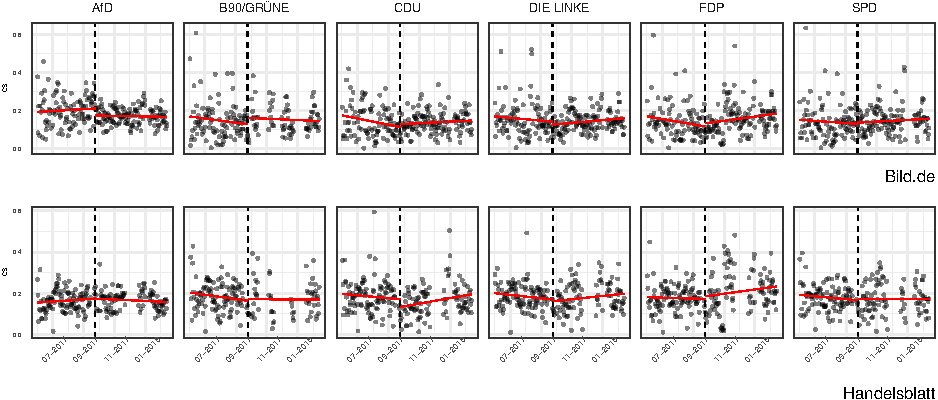
\includegraphics[width=0.9\linewidth]{main_text_files/figure-latex/Daily mean cosine similarity - rd example-1} 

}

\caption{Log of mean cosine similarity between newspaper/press articles pairs - with cutoff value \label{fig:mean_cosine_sim_rd_example}}\label{fig:Daily mean cosine similarity - rd example}
\end{figure}

In order to statistically evaluate these observations, two model
specifications are estimated for each news publisher: (1) First, a
simple regression discontinuity specification is estimated followed by
(2) a specification that includes dummy variables for parties to check
for differences in news publisher - party pairs.

\hypertarget{regression-discontinuity-rd-specification}{%
\subsubsection{Regression Discontinuity (RD)
specification}\label{regression-discontinuity-rd-specification}}

\emph{Todo:} - Define bandwidth - Write interpretation - use r package
for estimation (?)

A RD design is used to estimate the effects of the election day.
Specifically, I estimate the equation

\[
\ln(\text{CS}_{t})=\beta_0+\beta_1T_t+f(W_t)+\epsilon_t
\] where

\[
T_t = 
\begin{cases}
1, & \text{ if date } \geq \text{election date} \\
0, & \text{ if date } < \text{election date}
\end{cases}
\] and the running variable \(W_t\) is the time difference between date
\(i\) and the election date (in days), such that \(\beta_1\) is the
average treatment effect for observations with
\(W_t = \text{election date}\). In other words, \(\beta_1\) gives the
average change of the similarity between the content of news publisher
and press releases after the election day. Identification in the RD
model comes from assuming that the underlying, potentially endogenous
relationship between \(\epsilon_t\) and the date is eliminated by the
flexible function \(f(.)\). In particular, the relationship between
\(\epsilon_t\) and the date must not change discontinuously on or near
the election date.

Following
(\protect\hyperlink{ref-imbens_regression_2008}{\textbf{imbens\_regression\_2008?}})
I estimate a local linear regression of the form:

\[
\ln(\text{CS}_{t})=\beta_0+\beta_1T_t+\beta_2W_t+\beta_3W_t*T_t+\epsilon_t
\]

In this specification, the function \(f(W_t)\) is specified as
\(\beta_2W_t+\beta_3W_t*T_t\).

\autoref{table:results_rd1} shows the results of the estimation.

\begin{table}[!htbp] \centering    \caption{Results from the regression discontinuity model}    \label{table:results_rd1}  \resizebox{0.99\textwidth}{!}{\begin{tabular}{@{\extracolsep{5pt}}lccccccc}  \\[-1.8ex]\hline  \hline \\[-1.8ex]   & \multicolumn{7}{c}{\textit{Dependent variable:}} \\  \cline{2-8}  \\[-1.8ex] & \multicolumn{7}{c}{Cosine similarity of topic distribution} \\   & DIE WELT & stern.de & ZEIT ONLINE & Handelsblatt & FOCUS Online & Bild.de & SPIEGEL ONLINE \\  \\[-1.8ex] & (1) & (2) & (3) & (4) & (5) & (6) & (7)\\  \hline \\[-1.8ex]   treated & $-$0.122$^{***}$ & $-$0.106$^{**}$ & $-$0.141$^{**}$ & $-$0.155$^{***}$ & $-$0.045 & 0.015 & 0.053 \\    & (0.041) & (0.050) & (0.061) & (0.056) & (0.043) & (0.060) & (0.050) \\    & & & & & & & \\   X\_centered & $-$0.001$^{*}$ & $-$0.0005 & $-$0.002$^{***}$ & $-$0.0003 & $-$0.001 & $-$0.001 & $-$0.002$^{***}$ \\    & (0.0004) & (0.001) & (0.001) & (0.001) & (0.0005) & (0.001) & (0.001) \\    & & & & & & & \\   treatedTRUE:X\_centered & 0.002$^{***}$ & 0.003$^{***}$ & 0.002$^{**}$ & 0.002$^{***}$ & 0.001$^{**}$ & 0.002$^{**}$ & 0.002$^{***}$ \\    & (0.001) & (0.001) & (0.001) & (0.001) & (0.001) & (0.001) & (0.001) \\    & & & & & & & \\   Constant & $-$1.972$^{***}$ & $-$2.181$^{***}$ & $-$1.927$^{***}$ & $-$1.812$^{***}$ & $-$2.091$^{***}$ & $-$2.080$^{***}$ & $-$2.160$^{***}$ \\    & (0.029) & (0.035) & (0.045) & (0.042) & (0.032) & (0.045) & (0.037) \\    & & & & & & & \\  \hline \\[-1.8ex]  Observations & 1,372 & 1,378 & 1,404 & 1,206 & 1,428 & 1,321 & 1,424 \\  R$^{2}$ & 0.025 & 0.021 & 0.058 & 0.016 & 0.004 & 0.010 & 0.008 \\  Adjusted R$^{2}$ & 0.023 & 0.019 & 0.056 & 0.013 & 0.002 & 0.008 & 0.006 \\  Residual Std. Error & 0.373 (df = 1368) & 0.459 (df = 1374) & 0.578 (df = 1400) & 0.481 (df = 1202) & 0.415 (df = 1424) & 0.559 (df = 1317) & 0.479 (df = 1420) \\  F Statistic & 11.631$^{***}$ (df = 3; 1368) & 9.831$^{***}$ (df = 3; 1374) & 28.562$^{***}$ (df = 3; 1400) & 6.341$^{***}$ (df = 3; 1202) & 2.129$^{*}$ (df = 3; 1424) & 4.359$^{***}$ (df = 3; 1317) & 3.784$^{**}$ (df = 3; 1420) \\  \hline  \hline \\[-1.8ex]  \textit{Note:}  & \multicolumn{7}{r}{$^{*}$p$<$0.1; $^{**}$p$<$0.05; $^{***}$p$<$0.01} \\  \end{tabular}}  \end{table}

\hypertarget{rd-model-with-dummies}{%
\subsubsection{RD model with dummies}\label{rd-model-with-dummies}}

\emph{Todo:} - Define why we need the interaction term between treatment
+ dummy (find literature!)

Including interaction terms \(T_iD_{i,k-1}\) - and since we are
estimating an isolated model for each newspaper - \(\beta_4\) gives the
average treatment effect for each newspaper/party pair (i.e.~how how
much the slope changes for each party).

\[
\ln(\text{CS}_{i})=\beta_0+\beta_1T_i+\beta_2W_{i}+\beta_3D_{i,k-1}+\beta_4T_iD_{i,k-1}+\epsilon_i
\]

\begin{table}[!htbp] \centering    \caption{Results from the regression discontinuity model}    \label{table:results_rd2}  \resizebox{0.99\textwidth}{!}{\begin{tabular}{@{\extracolsep{5pt}}lccccccc}  \\[-1.8ex]\hline  \hline \\[-1.8ex]   & \multicolumn{7}{c}{\textit{Dependent variable:}} \\  \cline{2-8}  \\[-1.8ex] & \multicolumn{7}{c}{Cosine similarity of topic distribution} \\   & DIE WELT & stern.de & ZEIT ONLINE & Handelsblatt & FOCUS Online & Bild.de & SPIEGEL ONLINE \\  \\[-1.8ex] & (1) & (2) & (3) & (4) & (5) & (6) & (7)\\  \hline \\[-1.8ex]   treated & $-$0.149$^{**}$ & $-$0.090 & $-$0.113 & $-$0.089 & $-$0.100 & $-$0.189$^{**}$ & 0.047 \\    & (0.058) & (0.073) & (0.089) & (0.081) & (0.062) & (0.087) & (0.073) \\    & & & & & & & \\   X\_centered & 0.0002 & 0.001$^{***}$ & $-$0.001$^{**}$ & 0.001$^{***}$ & 0.0003 & 0.001 & $-$0.0003 \\    & (0.0003) & (0.0003) & (0.0004) & (0.0004) & (0.0003) & (0.0004) & (0.0003) \\    & & & & & & & \\   source2B90/GRÜNE & $-$0.267$^{***}$ & $-$0.216$^{***}$ & $-$0.180$^{**}$ & 0.105 & $-$0.338$^{***}$ & $-$0.445$^{***}$ & $-$0.187$^{***}$ \\    & (0.048) & (0.060) & (0.077) & (0.066) & (0.053) & (0.078) & (0.062) \\    & & & & & & & \\   source2CDU & $-$0.259$^{***}$ & $-$0.115$^{*}$ & $-$0.232$^{***}$ & 0.098 & $-$0.288$^{***}$ & $-$0.450$^{***}$ & $-$0.170$^{***}$ \\    & (0.048) & (0.060) & (0.077) & (0.066) & (0.053) & (0.078) & (0.062) \\    & & & & & & & \\   source2DIE LINKE & $-$0.251$^{***}$ & $-$0.109$^{*}$ & $-$0.160$^{**}$ & 0.134$^{**}$ & $-$0.270$^{***}$ & $-$0.342$^{***}$ & $-$0.156$^{**}$ \\    & (0.048) & (0.060) & (0.077) & (0.066) & (0.053) & (0.078) & (0.062) \\    & & & & & & & \\   source2FDP & $-$0.291$^{***}$ & $-$0.195$^{***}$ & $-$0.201$^{***}$ & 0.069 & $-$0.355$^{***}$ & $-$0.441$^{***}$ & $-$0.292$^{***}$ \\    & (0.048) & (0.060) & (0.077) & (0.066) & (0.053) & (0.078) & (0.062) \\    & & & & & & & \\   source2SPD & $-$0.278$^{***}$ & $-$0.143$^{**}$ & $-$0.201$^{***}$ & 0.098 & $-$0.339$^{***}$ & $-$0.479$^{***}$ & $-$0.266$^{***}$ \\    & (0.048) & (0.060) & (0.077) & (0.066) & (0.053) & (0.078) & (0.062) \\    & & & & & & & \\   treatedTRUE:source2B90/GRÜNE & 0.050 & $-$0.042 & $-$0.154 & $-$0.184$^{*}$ & 0.078 & 0.245$^{**}$ & $-$0.031 \\    & (0.071) & (0.089) & (0.112) & (0.102) & (0.077) & (0.110) & (0.091) \\    & & & & & & & \\   treatedTRUE:source2CDU & $-$0.030 & $-$0.175$^{**}$ & $-$0.090 & $-$0.204$^{**}$ & $-$0.022 & 0.178$^{*}$ & $-$0.131 \\    & (0.066) & (0.083) & (0.104) & (0.094) & (0.072) & (0.103) & (0.085) \\    & & & & & & & \\   treatedTRUE:source2DIE LINKE & $-$0.032 & $-$0.059 & $-$0.068 & $-$0.113 & $-$0.037 & 0.120 & $-$0.097 \\    & (0.066) & (0.083) & (0.104) & (0.094) & (0.072) & (0.103) & (0.085) \\    & & & & & & & \\   treatedTRUE:source2FDP & 0.084 & 0.109 & $-$0.002 & 0.024 & 0.137$^{*}$ & 0.260$^{**}$ & 0.134 \\    & (0.066) & (0.083) & (0.104) & (0.094) & (0.072) & (0.103) & (0.085) \\    & & & & & & & \\   treatedTRUE:source2SPD & 0.025 & $-$0.068 & $-$0.058 & $-$0.145 & 0.070 & 0.252$^{**}$ & $-$0.002 \\    & (0.067) & (0.084) & (0.105) & (0.095) & (0.072) & (0.104) & (0.086) \\    & & & & & & & \\   Constant & $-$1.689$^{***}$ & $-$1.956$^{***}$ & $-$1.692$^{***}$ & $-$1.816$^{***}$ & $-$1.780$^{***}$ & $-$1.647$^{***}$ & $-$1.900$^{***}$ \\    & (0.037) & (0.047) & (0.059) & (0.051) & (0.041) & (0.059) & (0.048) \\    & & & & & & & \\  \hline \\[-1.8ex]  Observations & 1,372 & 1,378 & 1,404 & 1,206 & 1,428 & 1,321 & 1,424 \\  R$^{2}$ & 0.091 & 0.045 & 0.080 & 0.023 & 0.080 & 0.059 & 0.043 \\  Adjusted R$^{2}$ & 0.083 & 0.037 & 0.072 & 0.013 & 0.072 & 0.050 & 0.035 \\  Residual Std. Error & 0.361 (df = 1359) & 0.455 (df = 1365) & 0.573 (df = 1391) & 0.481 (df = 1193) & 0.401 (df = 1415) & 0.547 (df = 1308) & 0.472 (df = 1411) \\  F Statistic & 11.334$^{***}$ (df = 12; 1359) & 5.354$^{***}$ (df = 12; 1365) & 10.113$^{***}$ (df = 12; 1391) & 2.335$^{***}$ (df = 12; 1193) & 10.240$^{***}$ (df = 12; 1415) & 6.847$^{***}$ (df = 12; 1308) & 5.310$^{***}$ (df = 12; 1411) \\  \hline  \hline \\[-1.8ex]  \textit{Note:}  & \multicolumn{7}{r}{$^{*}$p$<$0.1; $^{**}$p$<$0.05; $^{***}$p$<$0.01} \\  \end{tabular}}  \end{table}

Example interpretation for \emph{Bild.de} (see
\autoref{table:results_rd2})

The coefficient \(\beta_4\) for \(D_{SPD} = 1\) shows the difference of
the treatment effect for SPD. To illustrate this, we can compare the
model equation for \(D_{SPD} = 1\) and \(D_{SPD} = 0\)

\(D_{SPD} = 1\):
\(\begin{aligned} \ln(\text{CS})(D_{SPD}=1)=-1.647+(-0.189)T+(0.001)W-0.479+(0.252)T \\ \ln(\text{CS})(D_{SPD}=1)=-2,126+(0.001)W+(0.252-0.189)T \end{aligned}\)

\(D_{SPD} = 0\):
\(\begin{aligned} \ln(\text{CS})(D_{SPD}=0)=-1.647+(-0.189)T+(0.001)W \\ \ln(\text{CS})(D_{SPD}=0)=-1.647+(0.001)W+(-0.189)T \end{aligned}\)

\begin{itemize}
\tightlist
\item
  When \(D_{SPD}\) switches from 0 to 1, the treatment effect increases
  by \(0.252\).
\end{itemize}

To interpret this coefficient, we have to transform it (our dependent
variable is log transformed).

For \(D_{SPD} = 0\): \(\exp(-0.189)-1 = -0.172\)

After the election day the topic similarity between \emph{Bild.de} and
AfD decreased by \textasciitilde17.2\%

\(D_{SPD} = 1\): \(\exp(-0.189+0.252)-1 = 0.065\)

After the election day the topic similarity between \emph{Bild.de} and
SPD increased by \textasciitilde6.5\% compared to AfD.

General interpretation:

\begin{itemize}
\tightlist
\item
  News articles of \emph{DIE WELT} and \emph{Bild.de} show a significant
  decrease of topic similarity with AfD after the election. No such
  effect can be found for the other news papers.
\item
  News articles of \emph{Handelsblatt} are significantly less similar
  with B90/G \& CDU after the election (compared to AfD). The opposite
  is true for \emph{Bild.de} where new articles are more similar to ALL
  party press releases (except for DIE LINKE) when compared to AfD.
\end{itemize}

The results show, that for some news papers (\emph{DIE WELT} \&
\emph{Bild.de}), the there is a significant change in the topic
similarity between their news articles and the press releases of
parties.

\hypertarget{vi-discussion-and-conclusion}{%
\section{VI Discussion and
conclusion}\label{vi-discussion-and-conclusion}}

This paper investigates whether political reporting of news papers is
similar for all political parties. Results show, that the news articles
of all news papers (except for \emph{Handelsblatt}) are significantly
more similar to press releases of the AfD than any other party.

Furthermore, it was assumed, that this reporting differs between periods
of election campaign. The results show a significant effect of the
switch between ``before'' election (election campaign period) and
``after'' election for some news papers.

\begin{itemize}
\tightlist
\item
  For \emph{DIE WELT} and \emph{Bild.de} the election date has a
  significant effect on the similarity with the AfD: The similarity
  between news articles and press releases of AfD decreases
\end{itemize}

\newpage

\hypertarget{annex}{%
\section{Annex}\label{annex}}

\begin{longtable}[]{@{}lll@{}}
\caption{Online sources for press releases
\label{table:press_releases_sources}}\tabularnewline
\toprule
& Party & Parliamentary Group \\
\midrule
\endfirsthead
\toprule
& Party & Parliamentary Group \\
\midrule
\endhead
CDU & cdu.de & presseportal.de \\
SPD & spd.de & spdfraktion.de \\
FDP & fdp.de & fdpbt.de \\
B90/Die Grünen & gruene.de & gruene-bundestag.de \\
DIE LINKE & die-linke.de &
die-linke.de/start/presse/aus-dem-bundestag \\
AfD & afd.de & afdbundestag.de \\
\bottomrule
\end{longtable}

\% Table created by stargazer v.5.2.2 by Marek Hlavac, Harvard
University. E-mail: hlavac at fas.harvard.edu \% Date and time: So, Aug
15, 2021 - 18:33:22

\begin{table}[!htbp] \centering 
  \caption{7 most probable terms per topic} 
  \label{table:top_terms} 
\begin{tabular}{@{\extracolsep{5pt}} cc} 
\\[-1.8ex]\hline 
\hline \\[-1.8ex] 
 & Top Terms \\ 
\hline \\[-1.8ex] 
1 & a, the, s, of, u, brexit, großbritannien \\ 
2 & merkel, angela, kanzlerin, bundeskanzlerin, cdu, merkels, deutschland \\ 
3 & spd, union, cdu, csu, koalitionsvertrag, koalitionsverhandlungen, schulz \\ 
4 & afd, weidel, gauland, alice, alexander, politiker, äußerungen \\ 
5 & stimmen, wahlkreis, kandidaten, afd, wahl, gewählt, fdp \\ 
6 & trump, us, usa, deutschland, präsident, donald, berlin \\ 
7 & cdu, union, peter, politiker, spahn, altmaier, schäuble \\ 
8 & spd, koalition, union, groko, große, koalitionsverhandlungen, parteitag \\ 
9 & afd, partei, sachsen, gauland, parteien, pazderski, höcke \\ 
10 & diesel, unternehmen, deutschland, autos, deutschen, industrie, fahrverbote \\ 
11 & ge, ten, be, le, ver, lambsdorff, te \\ 
12 & gericht, prozess, urteil, richter, staatsanwaltschaft, verfahren, jahre \\ 
13 & berlin, deutschen, osten, o, tag, jahr, millionen \\ 
14 & august, cdu, spd, prozent, bundestagswahl, wahl, parteien \\ 
15 & kohl, helmut, kohls, einheit, kanzler, tod, deutschen \\ 
16 & spd, nahles, andrea, partei, scholz, schulz, schwesig \\ 
17 & csu, seehofer, horst, söder, obergrenze, bayern, chef \\ 
18 & prozent, umfrage, spd, union, fdp, cdu, afd \\ 
19 & polizei, stadt, menschen, polizisten, täter, verletzt, angaben \\ 
20 & euro, milliarden, jahr, millionen, prozent, bund, geld \\ 
21 & grünen, linke, linken, özdemir, partei, wagenknecht, göring \\ 
22 & cdu, niedersachsen, spd, grünen, rot, fdp, landtag \\ 
23 & welt, politik, menschen, jahren, lange, frage, fragen \\ 
24 & g, hamburg, gipfel, polizei, hamburger, demonstranten, scholz \\ 
25 & deutschland, is, verfassungsschutz, syrien, gefährder, islamisten, staat \\ 
26 & steinmeier, schmidt, russland, frank, bundespräsident, glyphosat, walter \\ 
27 & afd, petry, partei, fraktion, frauke, meuthen, gauland \\ 
28 & berliner, berlin, amri, maizière, innenminister, behörden, daten \\ 
29 & gabriel, sigmar, außenminister, spd, schröder, amt, gerhard \\ 
30 & bundestag, spd, abgeordneten, abgeordnete, parlament, abstimmung, fraktion \\ 
31 & türkei, erdogan, türkischen, deutschland, bundesregierung, türkische, deutsche \\ 
32 & frauen, deutschland, kinder, studie, eltern, muslime, antisemitismus \\ 
33 & fdp, jamaika, lindner, koalition, neuwahlen, spd, grünen \\ 
34 & facebook, maas, twitter, gesetz, internet, netz, heiko \\ 
35 & eu, deutschland, europa, bundesregierung, europäischen, deutschen, menschen \\ 
36 & bundeswehr, soldaten, leyen, nato, ursula, einsatz, verteidigungsministerin \\ 
37 & schulz, spd, martin, kanzlerkandidat, wahlkampf, bundestagswahl, partei \\ 
38 & flüchtlinge, deutschland, menschen, zahl, flüchtlingen, familiennachzug, jahr \\ 
39 & fdp, grünen, jamaika, csu, union, grüne, cdu \\ 
40 & bundestagswahl, afd, wahl, prozent, partei, bundestag, parteien \\ 
\hline \\[-1.8ex] 
\end{tabular} 
\end{table}

\begin{figure}

{\centering 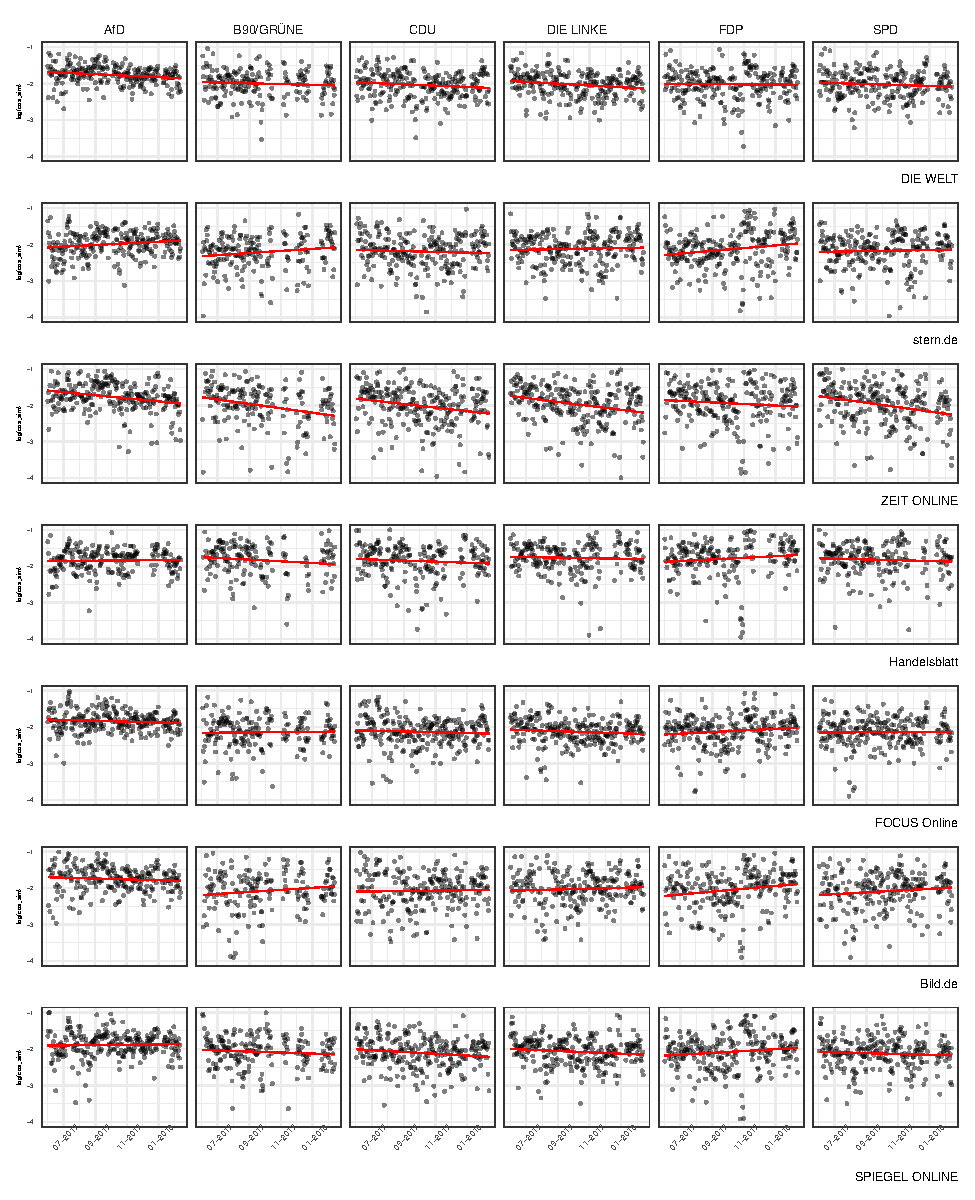
\includegraphics[width=1\linewidth]{main_text_files/figure-latex/Daily mean cosine similarity-1} 

}

\caption{Log of daily mean cosine similarity between newspaper/press articles pairs \label{fig:mean_cosine_sim_ols}}\label{fig:Daily mean cosine similarity}
\end{figure}

\begin{figure}

{\centering 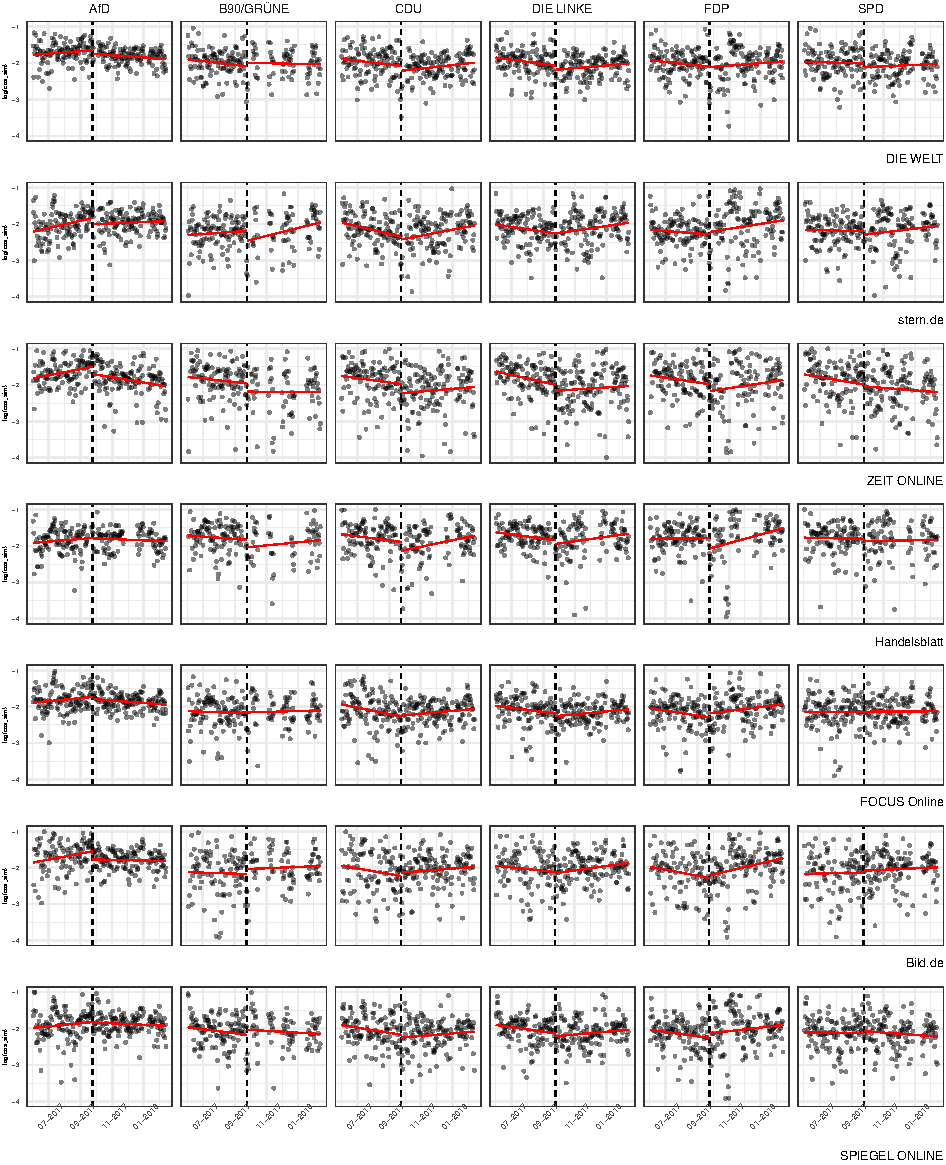
\includegraphics[width=1\linewidth]{main_text_files/figure-latex/Daily mean cosine similarity - cutoff value-1} 

}

\caption{Log of daily mean cosine similarity between newspaper/press articles pairs - with cutoff value \label{fig:mean_cosine_sim_rd}}\label{fig:Daily mean cosine similarity - cutoff value}
\end{figure}

\newpage

\hypertarget{references}{%
\section*{References}\label{references}}
\addcontentsline{toc}{section}{References}

\hypertarget{refs}{}
\begin{CSLReferences}{1}{0}
\leavevmode\hypertarget{ref-bholat_text_2015}{}%
Bholat, David M., Stephen Hansen, Pedro M. Santos, and Cheryl
Schonhardt-Bailey. 2015. {``Text Mining for Central Banks.''}
\emph{{SSRN} Electronic Journal}, June.
\url{http://www.academia.edu/13430482/Text_mining_for_central_banks}.

\leavevmode\hypertarget{ref-blassnig_hitting_2019}{}%
Blassnig, Sina, Sven Engesser, Nicole Ernst, and Frank Esser. 2019.
{``Hitting a Nerve: Populist News Articles Lead to More Frequent and
More Populist Reader Comments.''} \emph{Political Communication},
August, 1--23. \url{https://doi.org/10.1080/10584609.2019.1637980}.

\leavevmode\hypertarget{ref-blei_latent_2003}{}%
Blei, David M., Andrew Y Ng, and Michael I Jordan. 2003. {``Latent
Dirichlet Allocation.''} \emph{Journal of Machine Learning Research} 3
(January): 993--1022.

\leavevmode\hypertarget{ref-braun_variational_2010}{}%
Braun, Michael, and Jon McAuliffe. 2010. {``Variational Inference for
Large-Scale Models of Discrete Choice.''} \emph{Journal of the American
Statistical Association} 105 (489): 324--35.
\url{https://doi.org/10.1198/jasa.2009.tm08030}.

\leavevmode\hypertarget{ref-dewenter_einfuhrung_2014}{}%
Dewenter, Ralf, and Jürgen Rösch. 2014. \emph{Einführung in die neue
Ökonomie der Medienmärkte: Eine wettbewerbsökonomische Betrachtung aus
Sicht der Theorie der zweiseitigen Märkte}. Springer-Verlag.

\leavevmode\hypertarget{ref-druckman_impact_2005}{}%
Druckman, James N., and Michael Parkin. 2005. {``The Impact of Media
Bias: How Editorial Slant Affects Voters.''} \emph{The Journal of
Politics} 67 (4): 1030--49.
\url{https://doi.org/10.1111/j.1468-2508.2005.00349.x}.

\leavevmode\hypertarget{ref-eberl_lying_2018}{}%
Eberl, Jakob-Moritz. 2018. {``Lying Press: Three Levels of Perceived
Media Bias and Their Relationship with Political Preferences.''}
\emph{Communications}, March.
\url{https://doi.org/10.1515/commun-2018-0002}.

\leavevmode\hypertarget{ref-eberl_one_2017}{}%
Eberl, Jakob-Moritz, Hajo G. Boomgaarden, and Markus Wagner. 2017.
{``One Bias Fits All? Three Types of Media Bias and Their Effects on
Party Preferences.''} \emph{Communication Research} 44 (8): 1125--48.
\url{https://doi.org/10.1177/0093650215614364}.

\leavevmode\hypertarget{ref-erosheva_mixed-membership_2004}{}%
Erosheva, Elena, Stephen Fienberg, and John Lafferty. 2004.
{``Mixed-Membership Models of Scientific Publications.''}
\emph{Proceedings of the National Academy of Sciences} 101 (April):
5220--27. \url{https://doi.org/10.1073/pnas.0307760101}.

\leavevmode\hypertarget{ref-gentzkow_media_2004}{}%
Gentzkow, Matthew A., and Jesse M. Shapiro. 2004. {``Media, Education
and Anti-Americanism in the Muslim World.''} \emph{Journal of Economic
Perspectives} 18 (3): 117--33.
\url{https://doi.org/10.1257/0895330042162313}.

\leavevmode\hypertarget{ref-gentzkow_text_2017}{}%
Gentzkow, Matthew, Bryan T. Kelly, and Matt Taddy. 2017. {``Text as
Data.''} Working Paper 23276. National Bureau of Economic Research.
\url{https://doi.org/10.3386/w23276}.

\leavevmode\hypertarget{ref-griffiths_probabilistic_2002}{}%
Griffiths, Thomas L., and Mark Steyvers. 2002. {``A Probabilistic
Approach to Semantic Representation.''} \emph{Proceedings of the Annual
Meeting of the Cognitive Science Society} 24 (24).
\url{https://escholarship.org/uc/item/44x9v7m7}.

\leavevmode\hypertarget{ref-griffiths_finding_2004}{}%
---------. 2004. {``Finding Scientific Topics.''} \emph{Proceedings of
the National Academy of Sciences} 101 (April): 5228--35.
\url{https://doi.org/10.1073/pnas.0307752101}.

\leavevmode\hypertarget{ref-grimmer_text_2013}{}%
Grimmer, Justin, and Brandon Stewart. 2013. {``Text as Data: The Promise
and Pitfalls of Automatic Content Analysis Methods for Political
Texts.''} \emph{Political Analysis} 21: 267--97.

\leavevmode\hypertarget{ref-groseclose_measure_2005}{}%
Groseclose, Tim, and Jeffrey Milyo. 2005. {``A Measure of Media Bias.''}
\emph{The Quarterly Journal of Economics} 120 (4): 1191--1237.
\url{https://www.jstor.org/stable/25098770}.

\leavevmode\hypertarget{ref-hahn_identification_2001}{}%
Hahn, Jinyong, Petra Todd, and Wilbert Van der Klaauw. 2001.
{``Identification and Estimation of Treatment Effects with a
Regression-Discontinuity Design.''} \emph{Econometrica} 69 (1): 201--9.
\url{https://www.jstor.org/stable/2692190}.

\leavevmode\hypertarget{ref-hofmann_probabilistic_1999}{}%
Hofmann, Thomas. 1999. {``Probabilistic Latent Semantic Indexing.''} In
\emph{Proceedings of the 22Nd Annual International {ACM} {SIGIR}
Conference on Research and Development in Information Retrieval},
50--57. {SIGIR} '99. New York, {NY}, {USA}: {ACM}.
\url{https://doi.org/10.1145/312624.312649}.

\leavevmode\hypertarget{ref-kepplinger_einfluss_2004}{}%
Kepplinger, Hans Mathias, and Marcus Maurer. 2004. {``Der Einfluss Der
Pressemitteilungen Der Bundesparteien Auf Die Berichterstattung Im
Bundestagswahlkampf 2002.''} In \emph{Quo Vadis Public Relations? Auf
Dem Weg Zum Kommunikationsmanagement: Bestandsaufnahmen Und
Entwicklungen}, edited by Juliana Raupp and Joachim Klewes, 113--24.
Wiesbaden: {VS} Verlag für Sozialwissenschaften.
\url{https://doi.org/10.1007/978-3-322-83381-5_9}.

\leavevmode\hypertarget{ref-lott_is_2014}{}%
Lott, John R., and Kevin A. Hassett. 2014. {``Is Newspaper Coverage of
Economic Events Politically Biased?''} \emph{Public Choice} 160 (1):
65--108. \url{https://doi.org/10.1007/s11127-014-0171-5}.

\leavevmode\hypertarget{ref-mimno_optimizing_2011}{}%
Mimno, David, Hanna M. Wallach, Edmund Talley, Miriam Leenders, and
Andrew McCallum. 2011. {``Optimizing Semantic Coherence in Topic
Models.''} In \emph{Proceedings of the Conference on Empirical Methods
in Natural Language Processing}, 262--72. {EMNLP} '11. Stroudsburg,
{PA}, {USA}: Association for Computational Linguistics.
\url{http://dl.acm.org/citation.cfm?id=2145432.2145462}.

\leavevmode\hypertarget{ref-newman_automatic_2010}{}%
Newman, David, Jey Han Lau, Karl Grieser, and Timothy Baldwin. 2010.
{``Automatic Evaluation of Topic Coherence.''} In \emph{Human Language
Technologies: The 2010 Annual Conference of the North American Chapter
of the Association for Computational Linguistics}, 100--108. {HLT} '10.
Stroudsburg, {PA}, {USA}: Association for Computational Linguistics.
\url{http://dl.acm.org/citation.cfm?id=1857999.1858011}.

\leavevmode\hypertarget{ref-newman_reuters_2018}{}%
Newman, Nic, Richard Fletcher, Antonis Kalogeropoulos, David Levy, and
Rasmus Kleis Nielsen. 2018. {``Reuters Institute Digital News Report
2018.''} Reuters Institute for the Study of Journalism.
\url{http://media.digitalnewsreport.org/wp-content/uploads/2018/06/digital-news-report-2018.pdf?x89475}.

\leavevmode\hypertarget{ref-ramage_characterizing_2010}{}%
Ramage, Daniel, Susan Dumais, and Daniel Liebling. 2010.
\emph{Characterizing Microblogs with Topic Models}.

\leavevmode\hypertarget{ref-rehs_structural_2020}{}%
Rehs, Andreas. 2020. {``A Structural Topic Model Approach to Scientific
Reorientation of Economics and Chemistry After German Reunification.''}
\emph{Scientometrics} 125 (2): 1229--51.
\url{https://doi.org/10.1007/s11192-020-03640-0}.

\leavevmode\hypertarget{ref-roberts_model_2016}{}%
Roberts, Margaret E., Brandon M. Stewart, and Edoardo M. Airoldi. 2016.
{``A Model of Text for Experimentation in the Social Sciences.''}
\emph{Journal of the American Statistical Association} 111 (515):
988--1003. \url{https://doi.org/10.1080/01621459.2016.1141684}.

\leavevmode\hypertarget{ref-roberts_navigating_2016}{}%
Roberts, Margaret, Brandon Stewart, and Dustin Tingley. 2016a.
{``Navigating the Local Modes of Big Data: The Case of Topic Models.''}
In \emph{Computational Social Science: Discovery and Prediction}. New
York: Cambridge University Press.

\leavevmode\hypertarget{ref-roberts_stm:_2016}{}%
---------. 2016b. {``Stm: R Package for Structural Topic Models.''}
\emph{Journal of Statistical Software} forthcoming (December).

\leavevmode\hypertarget{ref-stromback_four_2008}{}%
Strömbäck, Jesper. 2008. {``Four Phases of Mediatization: An Analysis of
the Mediatization of Politics.''} \emph{The International Journal of
Press/Politics} 13 (3): 228--46.
\url{https://doi.org/10.1177/1940161208319097}.

\leavevmode\hypertarget{ref-taddy_estimation_2012}{}%
Taddy, Matt. 2012. {``On Estimation and Selection for Topic Models.''}
In \emph{Proceedings of the 15th International Conference on Artificial
Intelligence and Statistics}.

\leavevmode\hypertarget{ref-takens_media_2013}{}%
Takens, Janet, Wouter Atteveldt, Anita van Hoof, and Jan Kleinnijenhuis.
2013. {``Media Logic in Election Campaign Coverage.''} \emph{European
Journal of Communication} 28 (June): 277--93.
\url{https://doi.org/10.1177/0267323113478522}.

\leavevmode\hypertarget{ref-thistlethwaite_regression-discontinuity_1960}{}%
Thistlethwaite, Donald L., and Donald T. Campbell. 1960.
{``Regression-Discontinuity Analysis: An Alternative to the Ex Post
Facto Experiment.''} \emph{Journal of Educational Psychology} 51 (6):
309--17. \url{https://doi.org/10.1037/h0044319}.

\leavevmode\hypertarget{ref-wallach_rethinking_2009}{}%
Wallach, Hanna M., David M. Mimno, and Andrew McCallum. 2009.
{``Rethinking {LDA}: Why Priors Matter.''} In \emph{Advances in Neural
Information Processing Systems 22}, edited by Y. Bengio, D. Schuurmans,
J. D. Lafferty, C. K. I. Williams, and A. Culotta, 1973--81. Curran
Associates, Inc.
\url{http://papers.nips.cc/paper/3854-rethinking-lda-why-priors-matter.pdf}.

\end{CSLReferences}

\end{document}
